\chapter{Mockups de Interfaces del Sistema}
\label{anexo:Mockups}
---------------------------------------------------------------------------
\begin{appendices}

    
    \section{Perfil: Quejoso}
    \label{sec:mockups_quejoso}
    
    Los mockups presentados en esta sección representan el diseño visual de la interfaz de usuario del Quejoso. Las vistas se organizan en el orden recomendado de navegación del quejoso: desde el punto de entrada al portal, pasando por el registro y autenticación, hasta la gestión de expedientes y propuestas de conciliación.
    
    % ---- MQ-01 ----
    \subsection{MQ-01: Pantalla de Inicio}
    
    Es el punto de acceso principal para la comunidad politécnica. Presenta una interfaz limpia con tres acciones principales: presentar una nueva queja, dar seguimiento a un trámite existente como invitado, o iniciar sesión. Incluye elementos informativos sobre los derechos y el propósito de la Defensoría.
    
    \begin{figure}[H]
        \centering
        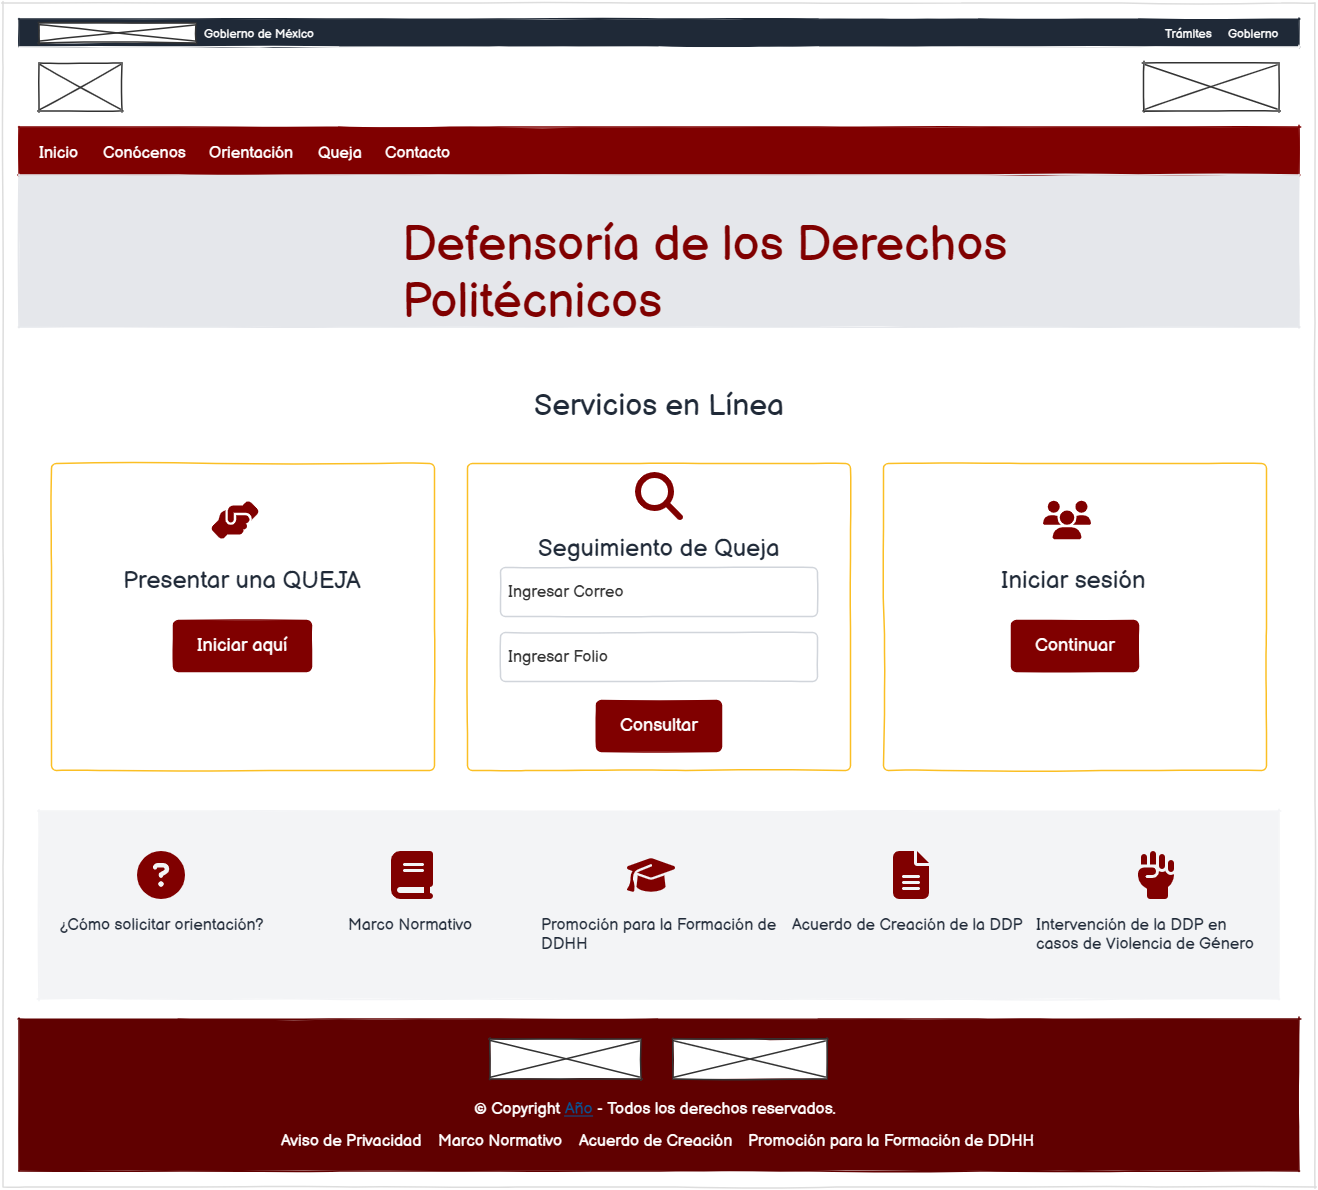
\includegraphics[width=0.80\textwidth, height=0.70\textheight, keepaspectratio]{imagenes/quejoso/Mockups/MQ-01_PantallaInicio.png}
        \caption{Mockup MQ-01: Pantalla de Inicio del Portal}
        \label{fig:mq01_pantalla_inicio}
    \end{figure}
    
    % ---- MQ-02 ----
    \subsection{MQ-02: Formulario de Registro de Queja}
    
    Interfaz diseñada para la captura de información de una queja. Se divide en secciones lógicas: datos personales del quejoso, narrativa detallada de los hechos y un área de carga de archivos multimedia para las evidencias. Utiliza validaciones para asegurar que los campos obligatorios sean completados correctamente.
    
    \begin{figure}[H]
        \centering
        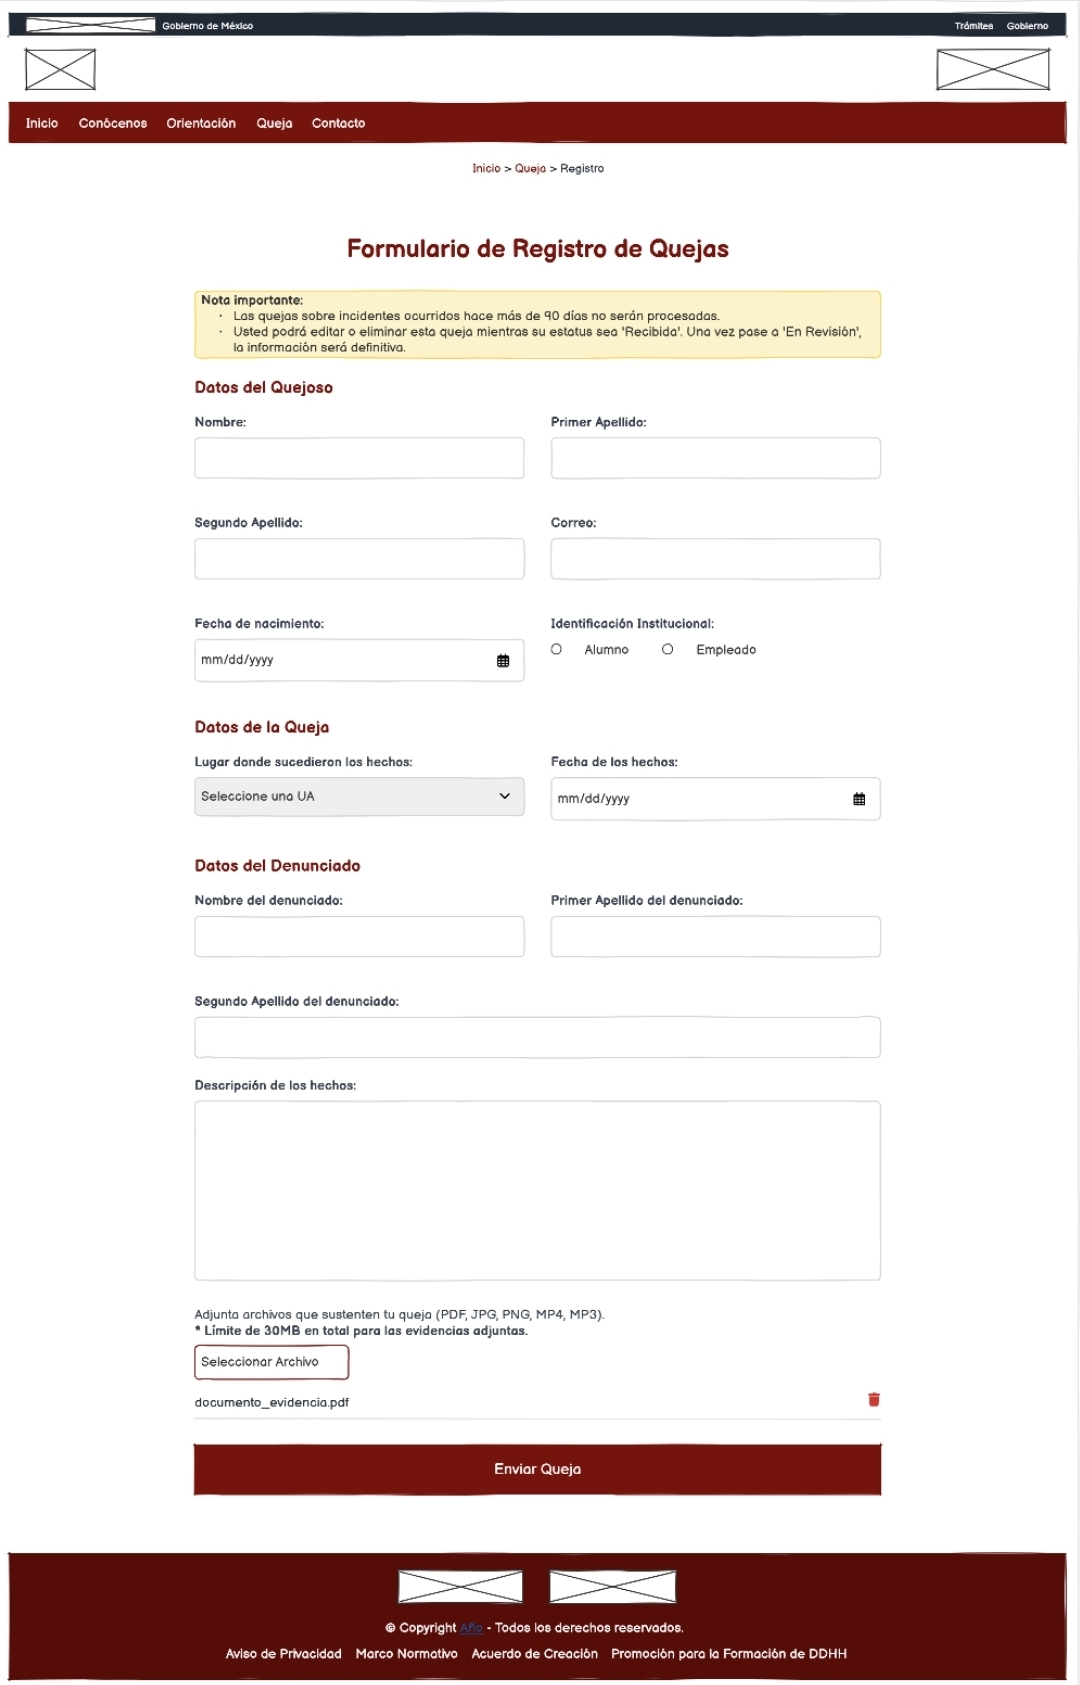
\includegraphics[width=0.80\textwidth, height=0.70\textheight, keepaspectratio]{imagenes/quejoso/Mockups/MQ-02_FormularioRegistro.jpg}
        \caption{Mockup MQ-02: Formulario de Registro de Queja}
        \label{fig:mq02_formulario_registro}
    \end{figure}
    
    % ---- MQ-03 ----
    \subsection{MQ-03: Ventana de Datos del Tutor}
    
    Componente modal que se activa automáticamente cuando el sistema detecta que el quejoso es menor de edad basándose en su fecha de nacimiento. Solicita los datos de contacto y parentesco de un adulto responsable para proceder con la validez jurídica del trámite.
    
    \begin{figure}[H]
        \centering
        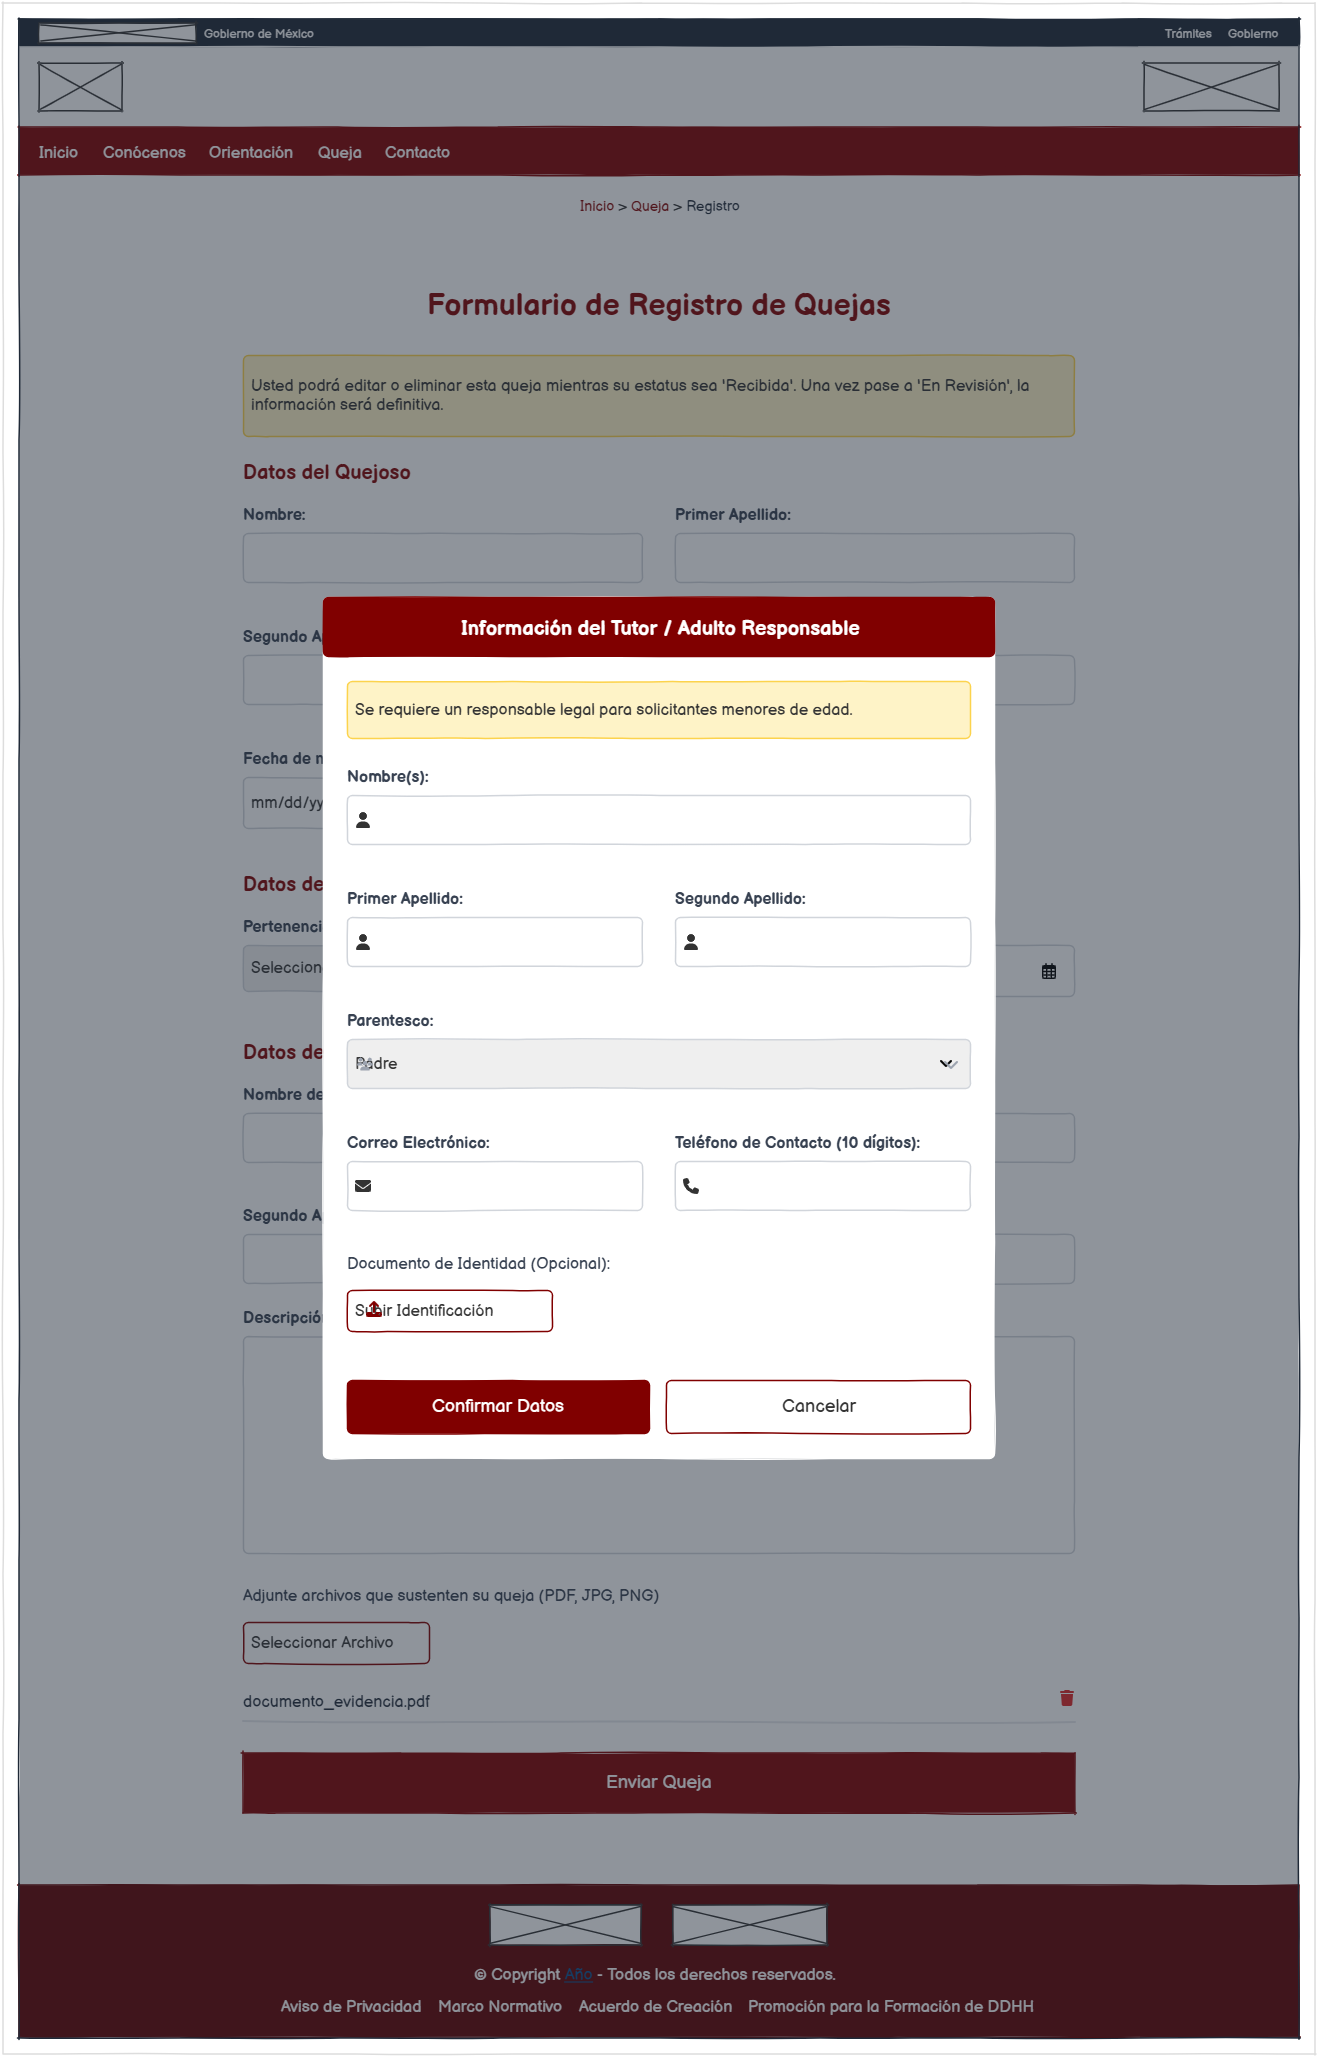
\includegraphics[width=0.80\textwidth, height=0.70\textheight, keepaspectratio]{imagenes/quejoso/Mockups/MQ-03_VentanaTutor.png}
        \caption{Mockup MQ-03: Ventana de Datos del Tutor}
        \label{fig:mq03_ventana_tutor}
    \end{figure}
    
    % ---- MQ-04 ----
    \subsection{MQ-04: Pantalla de Éxito y Folio}
    
    Vista de confirmación tras el envío exitoso de la queja. Muestra el folio único de seguimiento generado por el sistema. Ofrece al usuario dos vías de acción inmediata: descargar el acuse de recibo en formato PDF o proceder a la configuración de una cuenta para seguimiento detallado.
    
    \begin{figure}[H]
        \centering
        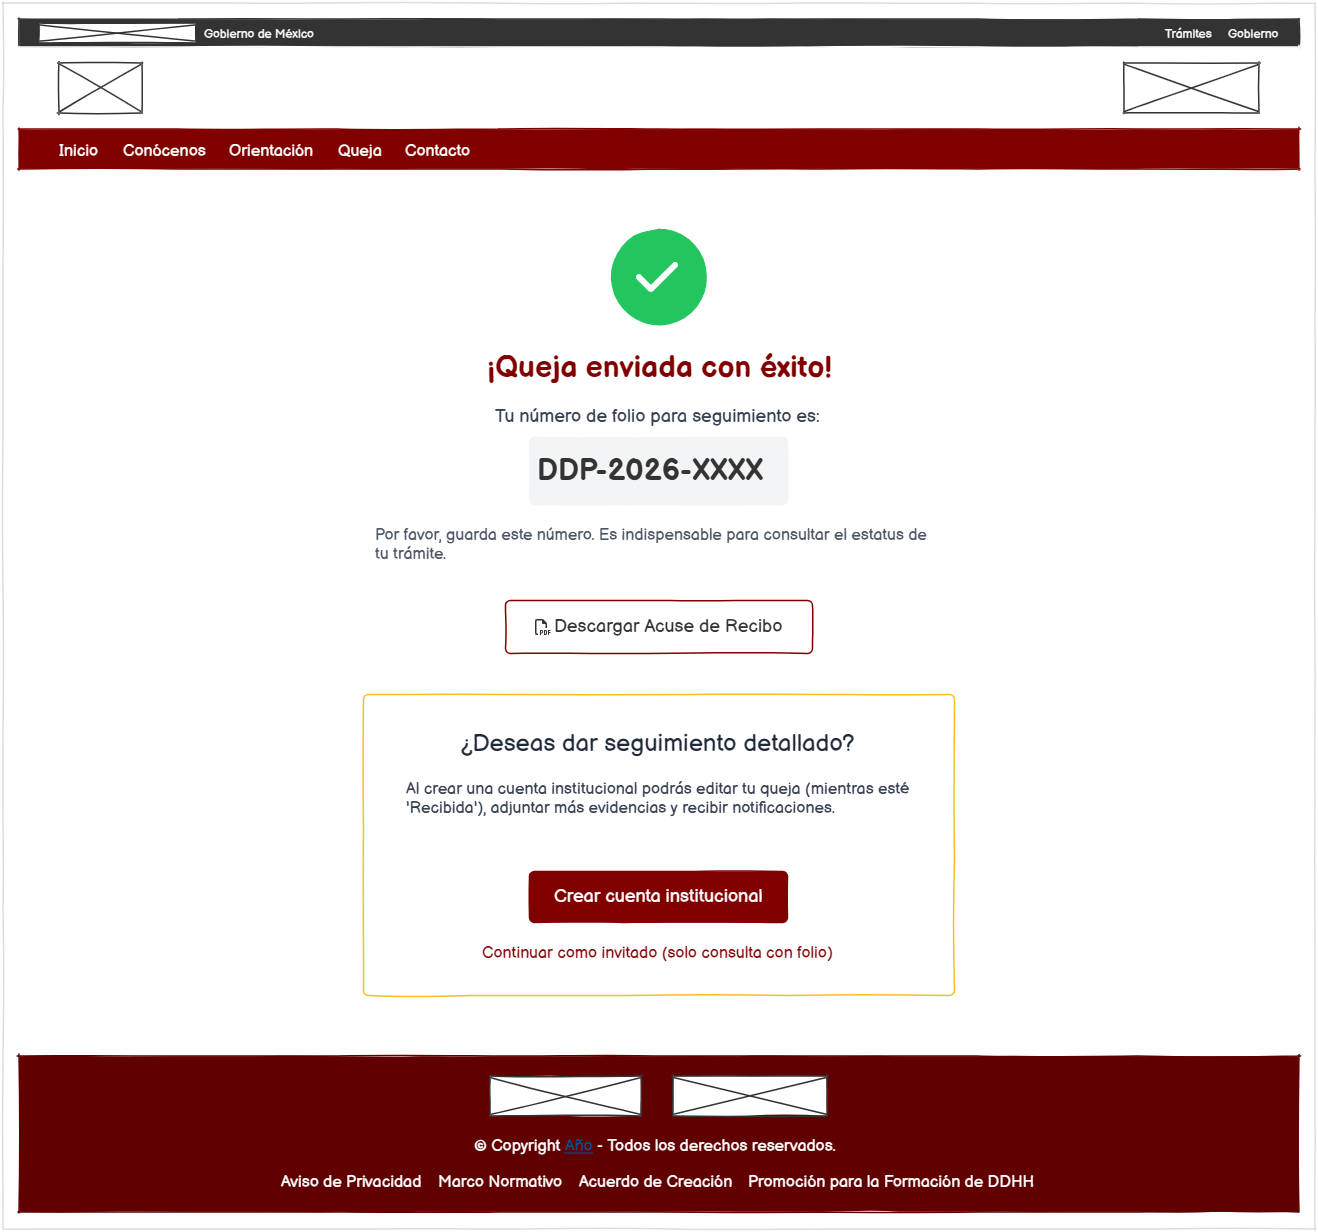
\includegraphics[width=0.80\textwidth, height=0.70\textheight, keepaspectratio]{imagenes/quejoso/Mockups/MQ-04_ExitoFolio.png}
        \caption{Mockup MQ-04: Pantalla de Éxito con Folio Generado}
        \label{fig:mq04_exito_folio}
    \end{figure}
    
    % ---- MQ-05 ----
    \subsection{MQ-05: Configuración de Cuenta}
    
    Pantalla dedicada a la transición de usuario invitado a registrado. Permite al quejoso establecer una contraseña de acceso segura vinculada al correo proporcionado en el registro. Es el paso previo para habilitar el acceso al Dashboard institucional.
    
    \begin{figure}[H]
        \centering
        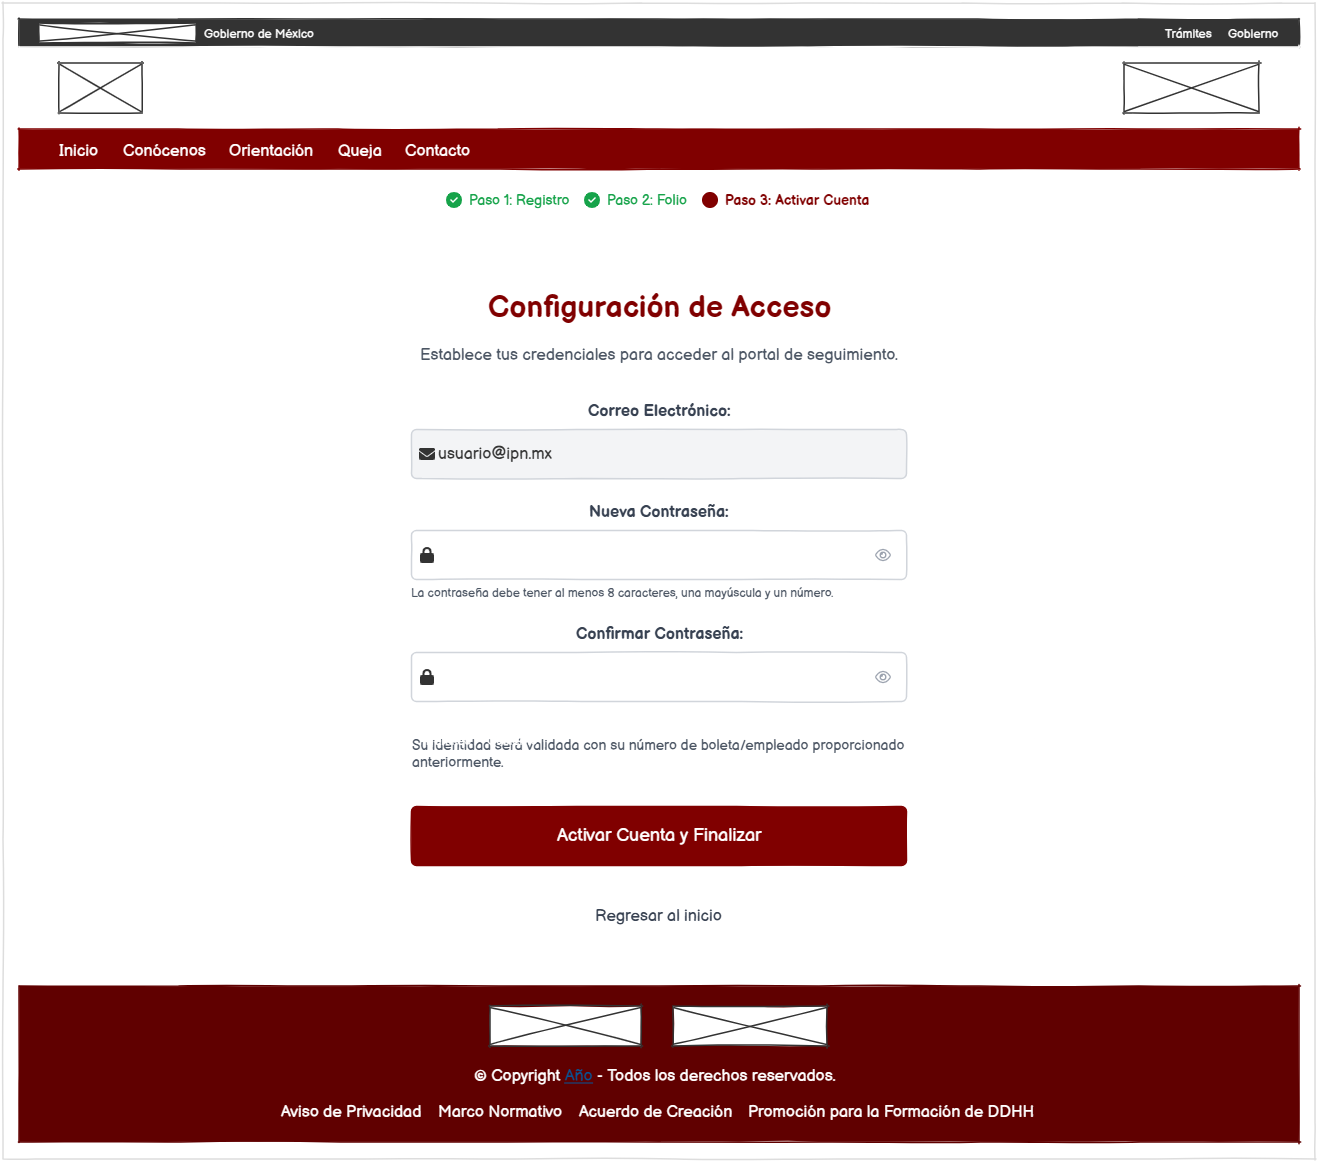
\includegraphics[width=0.80\textwidth, height=0.70\textheight, keepaspectratio]{imagenes/quejoso/Mockups/MQ-05_ConfiguracionCuenta.png}
        \caption{Mockup MQ-05: Configuración de Cuenta de Seguimiento}
        \label{fig:mq05_configuracion_cuenta}
    \end{figure}
    
    % ---- MQ-06 ----
    \subsection{MQ-06: Seguimiento sin Cuenta}
    
    Interfaz simplificada para el seguimiento de trámites sin necesidad de iniciar sesión. Permite a los usuarios que optaron por no crear una cuenta verificar el estatus de su trámite ingresando únicamente el folio y el correo electrónico asociado. Ofrece una vista resumida del estado actual del expediente, proporcionando información clave como la etapa administrativa y evidencias.
    
    \begin{figure}[H]
        \centering
        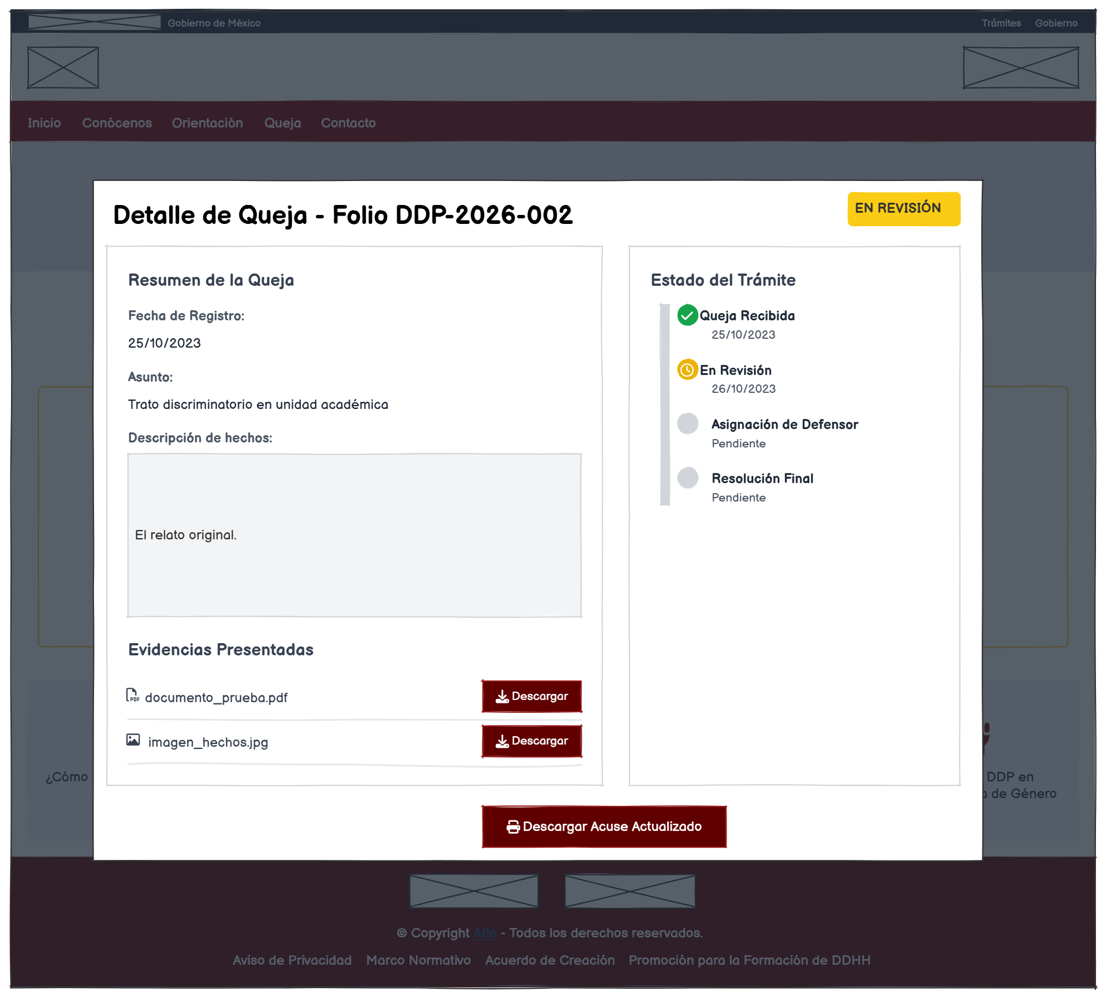
\includegraphics[width=0.80\textwidth, height=0.70\textheight, keepaspectratio]{imagenes/quejoso/Mockups/MQ-06_SeguimientoSinCuenta.png}
        \caption{Mockup MQ-06: Seguimiento de Expediente sin Cuenta}
        \label{fig:mq06_seguimiento_sin_cuenta}
    \end{figure}
    
    % ---- MQ-07 ----
    \subsection{MQ-07: Inicio de Sesión}
    
    Pantalla de inicio de sesión donde el usuario ingresa sus credenciales (correo y contraseña). Incluye controles de seguridad y un enlace directo para el proceso de recuperación de cuenta en caso de olvido de credenciales.
    
    \begin{figure}[H]
        \centering
        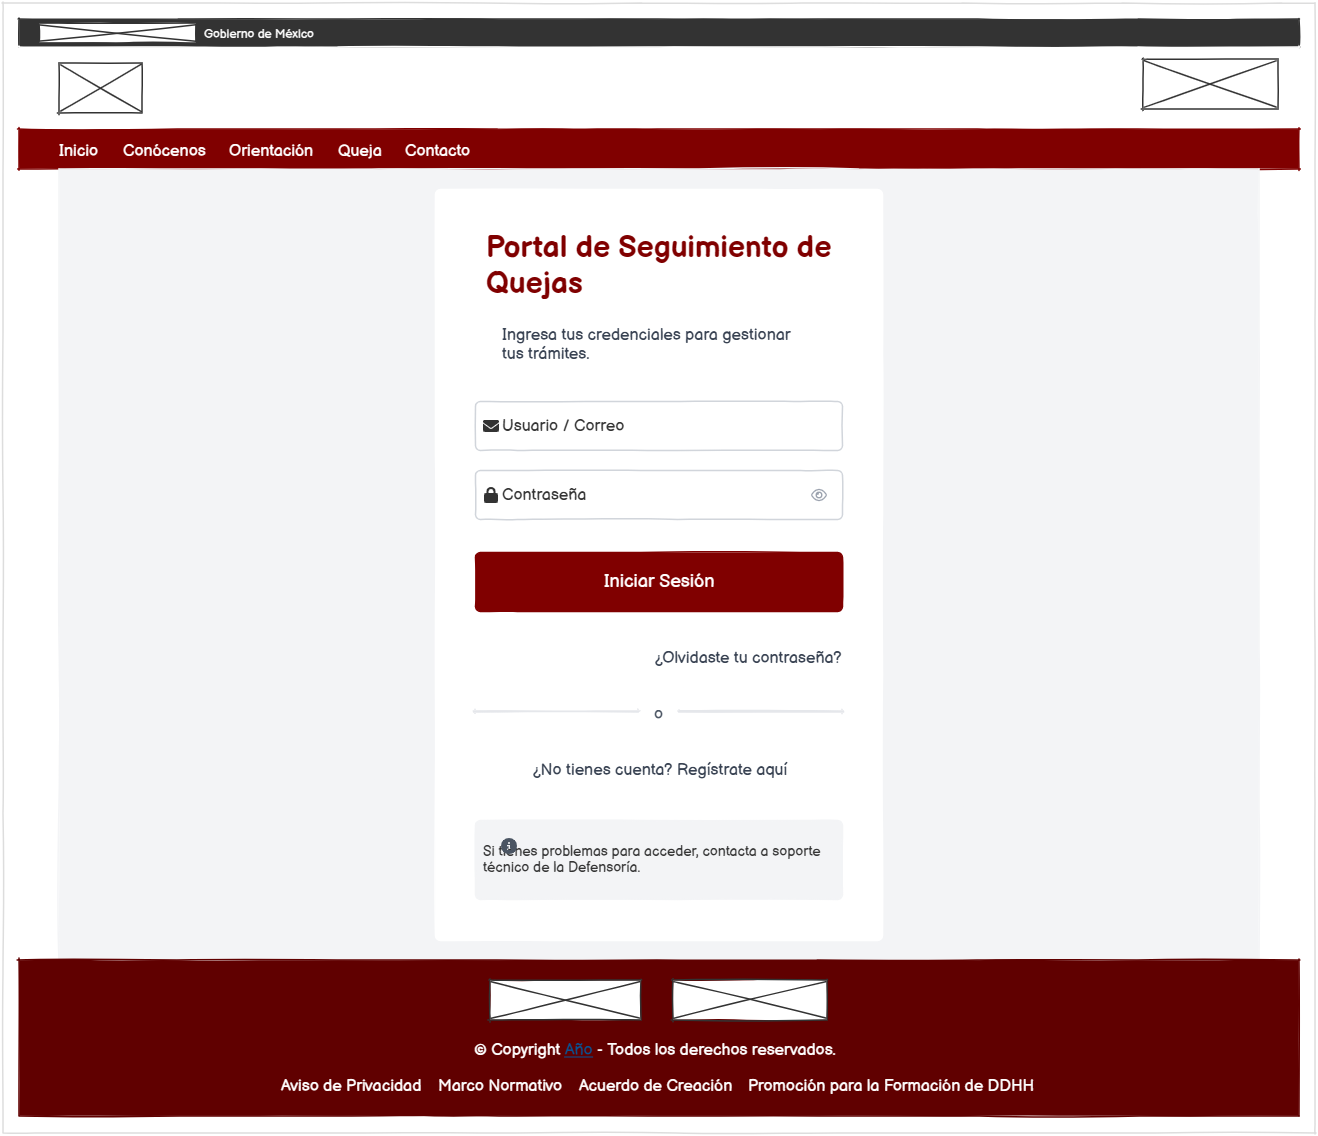
\includegraphics[width=0.80\textwidth, height=0.70\textheight, keepaspectratio]{imagenes/quejoso/Mockups/MQ-07_InicioSesionQuejoso.png}
        \caption{Mockup MQ-07: Pantalla de Inicio de Sesión}
        \label{fig:mq07_inicio_sesion}
    \end{figure}
    
    % ---- MQ-08 ----
    \subsection{MQ-08: Opciones de Cuenta}
    
    Pantalla de decisión que asiste al usuario que no cuenta con acceso. Ofrece dos rutas claras: iniciar el registro de una nueva queja desde cero o activar una cuenta de seguimiento utilizando un folio que ya le fue asignado previamente.
    
    \begin{figure}[H]
        \centering
        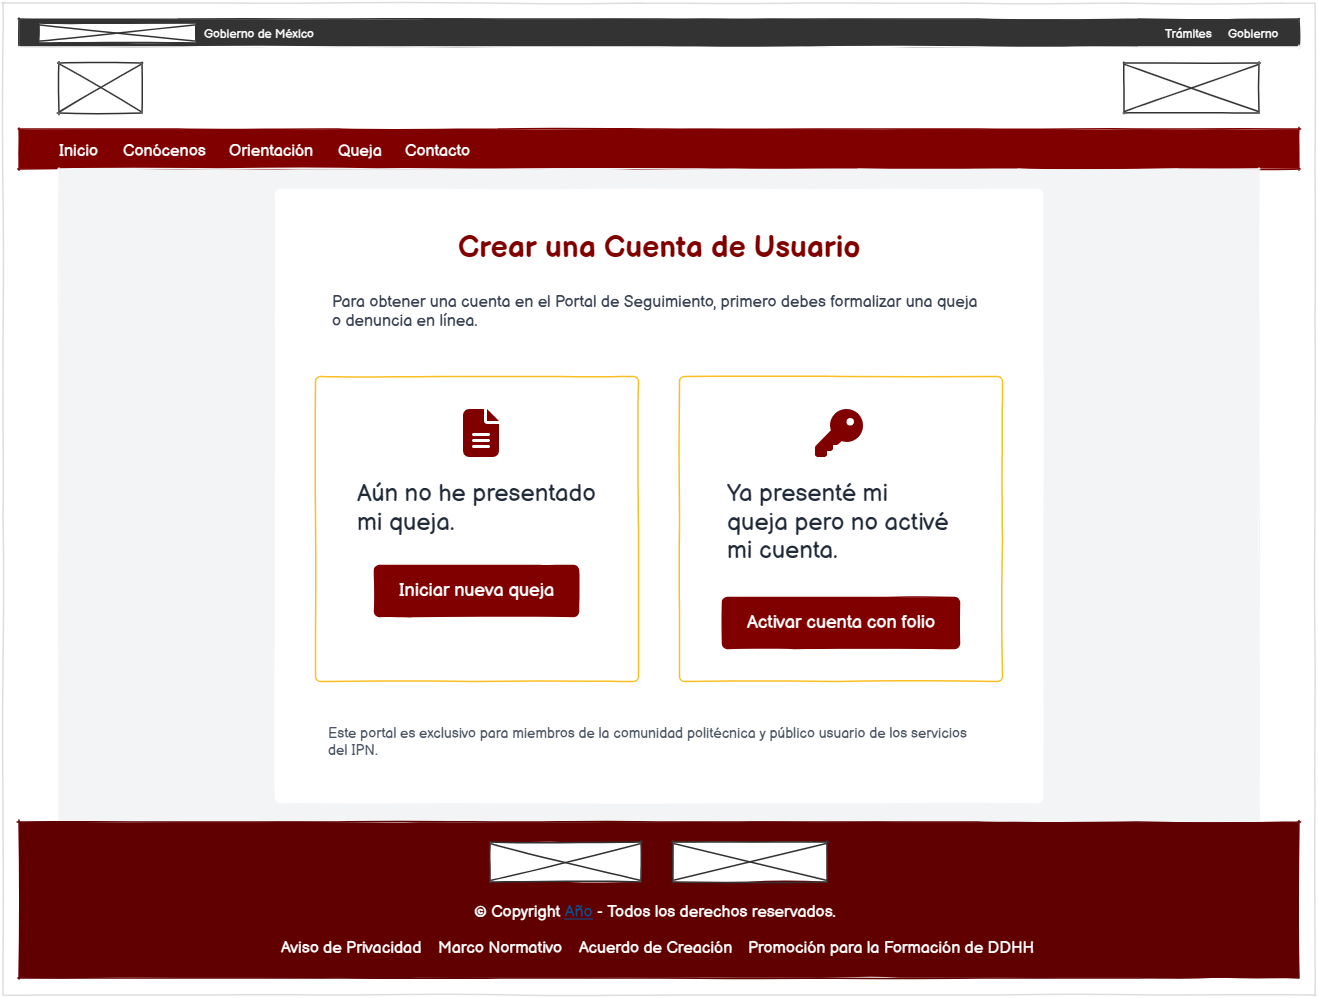
\includegraphics[width=0.80\textwidth, height=0.70\textheight, keepaspectratio]{imagenes/quejoso/Mockups/MQ-08_OpcionesCuenta.png}
        \caption{Mockup MQ-08: Opciones de Activación de Cuenta}
        \label{fig:mq08_opciones_cuenta}
    \end{figure}
    
    % ---- MQ-09 ----
    \subsection{MQ-09: Cuenta Existente}
    
    Interfaz de validación para usuarios que ya tienen un trámite en curso pero aún no han activado su perfil. Solicita el folio y el correo para verificar la identidad del solicitante en la base de datos antes de permitirle definir su contraseña de acceso.
    
    \begin{figure}[H]
        \centering
        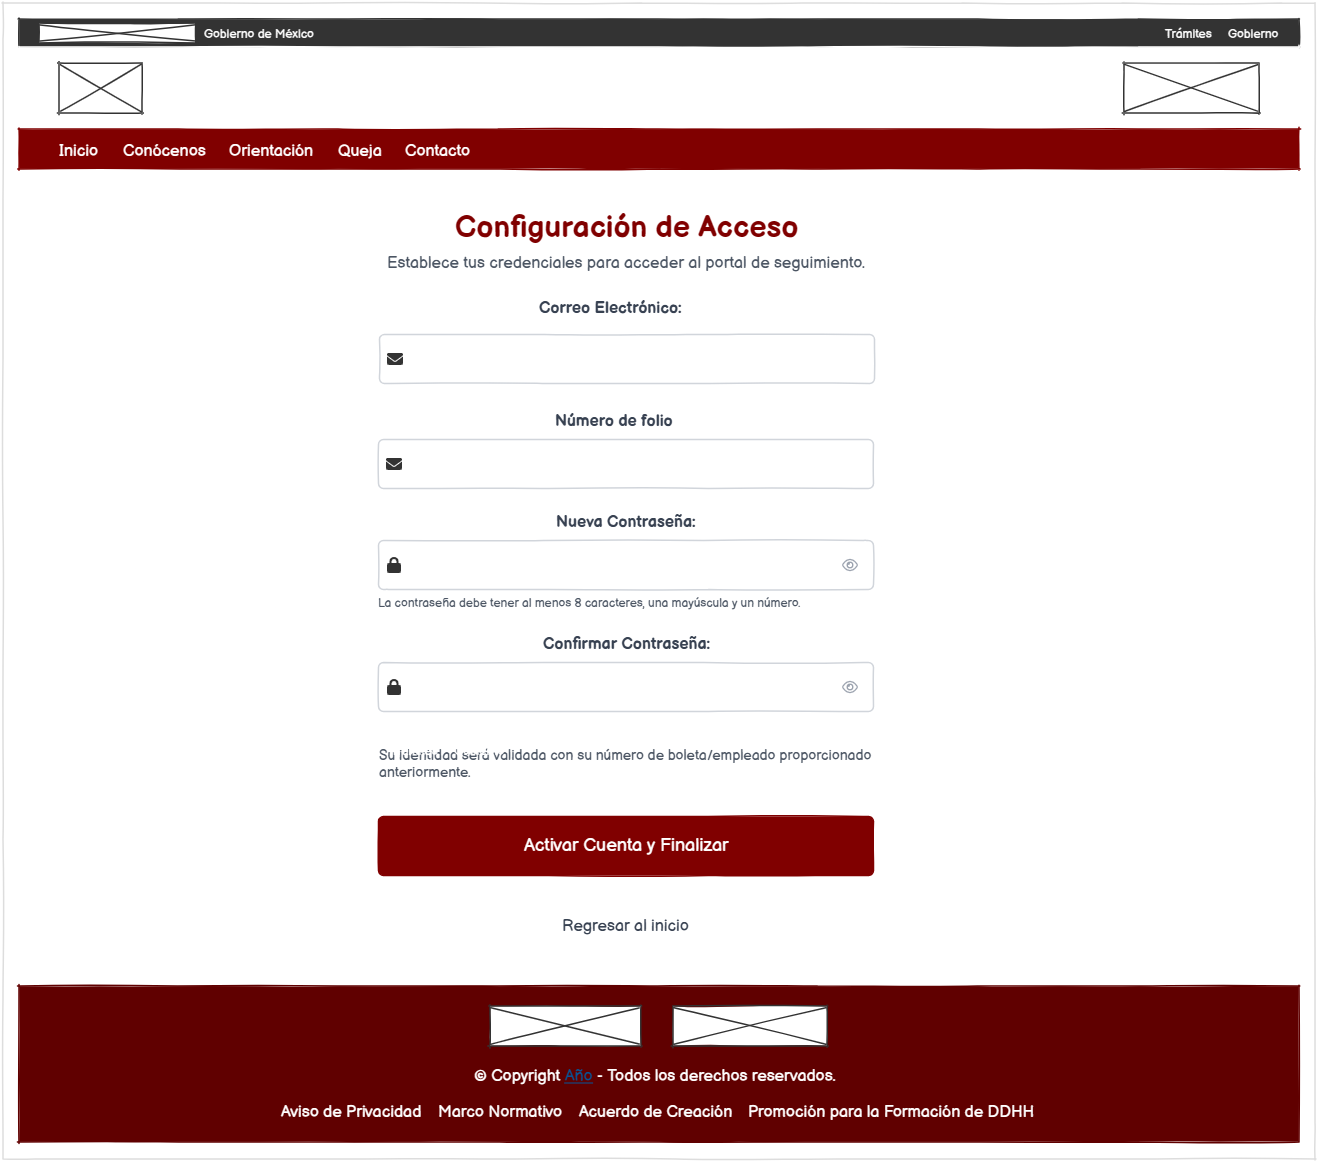
\includegraphics[width=0.80\textwidth, height=0.70\textheight, keepaspectratio]{imagenes/quejoso/Mockups/MQ-09_CuentaExistente.png}
        \caption{Mockup MQ-09: Aviso de Cuenta Existente}
        \label{fig:mq09_cuenta_existente}
    \end{figure}
    
    % ---- MQ-10 ----
    \subsection{MQ-10: Restablecer Contraseña}
    
    Flujo de recuperación de cuenta. Permite al usuario solicitar un enlace de restablecimiento mediante su correo electrónico registrado. Una vez validado el token, la interfaz habilita los campos para la creación y confirmación de la nueva credencial de acceso.
    
    \begin{figure}[H]
        \centering
        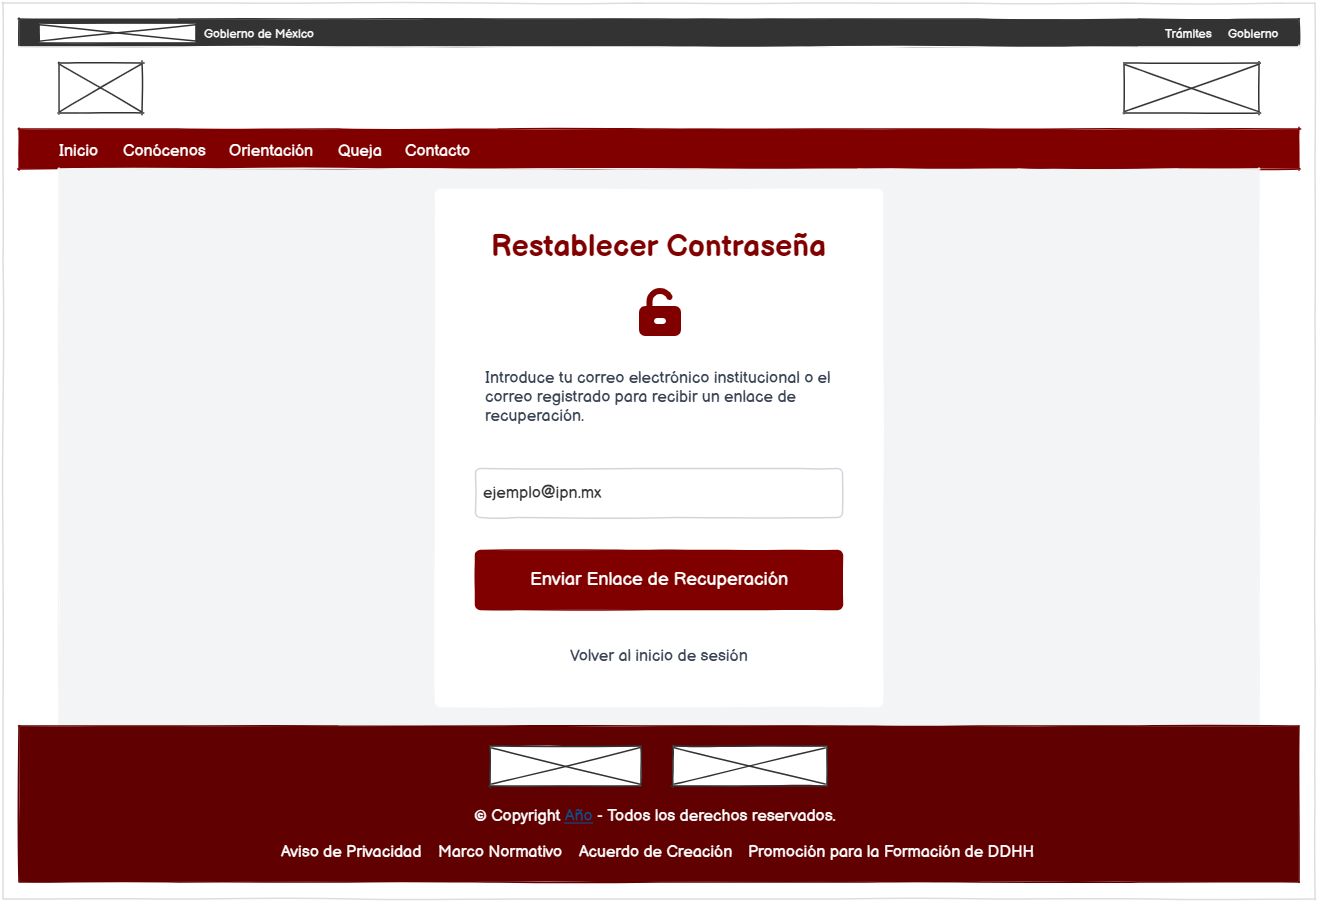
\includegraphics[width=0.80\textwidth, height=0.70\textheight, keepaspectratio]{imagenes/quejoso/Mockups/MQ-10_RestablecerPass.png}
        \caption{Mockup MQ-10: Pantalla de Restablecimiento de Contraseña}
        \label{fig:mq10_restablecer_pass}
    \end{figure}
    
    % ---- MQ-11 ----
    \subsection{MQ-11: Gestión de Trámites (Dashboard)}
    
    Representa la vista principal del usuario autenticado. Presenta un resumen ejecutivo con tarjetas de conteo estadístico sobre el estatus de sus quejas (Recibidas, En Revisión, Concluidas) y una tabla con los trámites más recientes, facilitando el acceso rápido a las acciones de edición, visualización o eliminación.
    
    \begin{figure}[H]
        \centering
        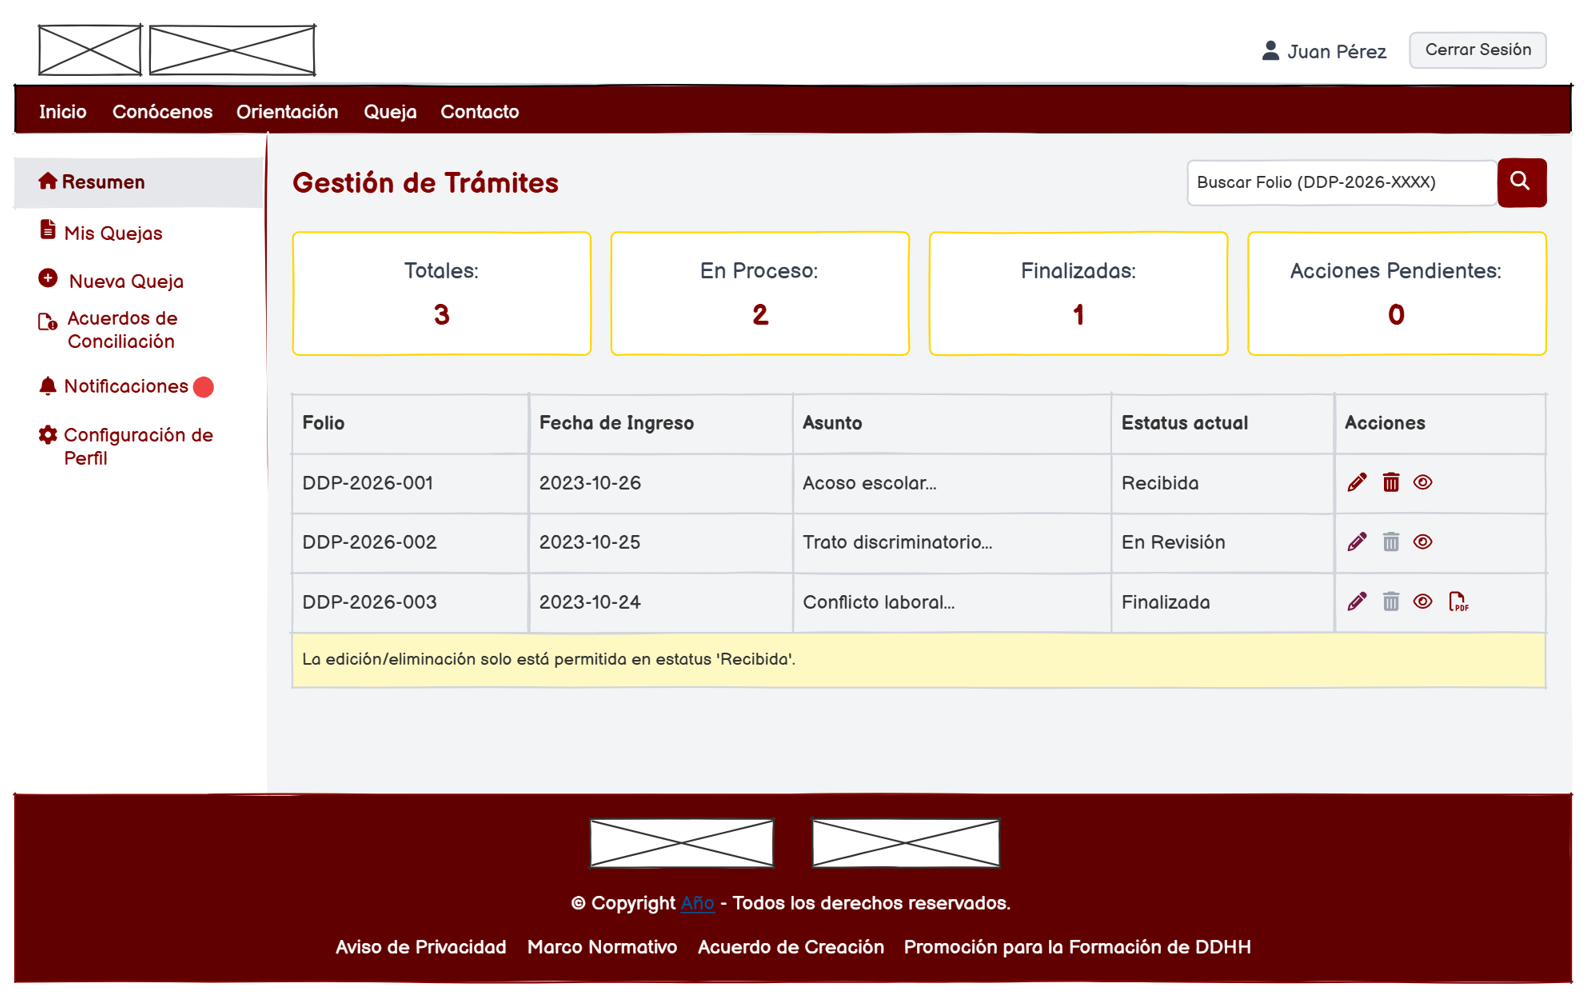
\includegraphics[width=0.80\textwidth, height=0.70\textheight, keepaspectratio]{imagenes/quejoso/Mockups/MQ-11_GestionTramites.png}
        \caption{Mockup MQ-11: Dashboard de Gestión de Trámites}
        \label{fig:mq11_gestion_tramites}
    \end{figure}
    
    % ---- MQ-12 ----
    \subsection{MQ-12: Confirmar Eliminación}
    
    Interfaz de diálogo modal diseñada para la eliminacion de una queja. Antes de procesar la cancelación lógica de un expediente, el sistema presenta una advertencia de seguridad para evitar eliminaciones accidentales. Esta opción solo se habilita si la queja se encuentra estrictamente en estatus "RECIBIDA".
    
    \begin{figure}[H]
        \centering
        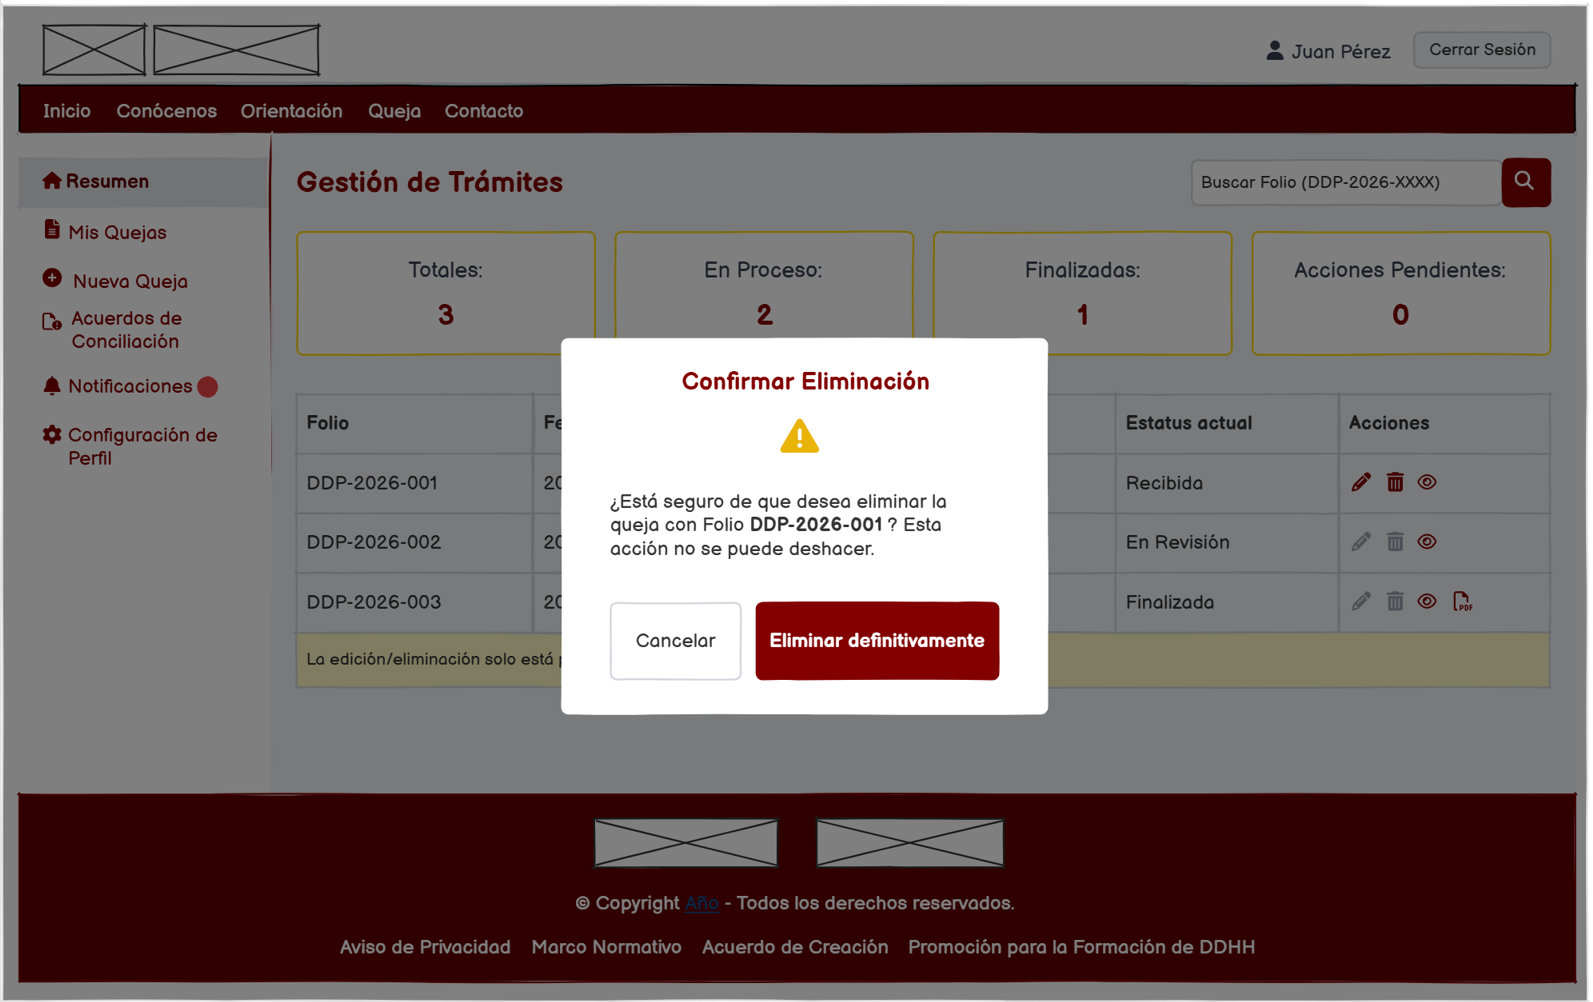
\includegraphics[width=0.80\textwidth, height=0.70\textheight, keepaspectratio]{imagenes/quejoso/Mockups/MQ-12_ConfirmarEliminacion.png}
        \caption{Mockup MQ-12: Diálogo de Confirmación de Eliminación}
        \label{fig:mq12_confirmar_eliminacion}
    \end{figure}
    
    % ---- MQ-13 ----
    \subsection{MQ-13: Editar Queja}
    
    Pantalla que permite al quejoso actualizar la información de su expediente. La interfaz carga los datos previamente registrados en el formulario, permitiendo modificar la narrativa de los hechos y gestionar los archivos de evidencia.
    
    \begin{figure}[H]
        \centering
        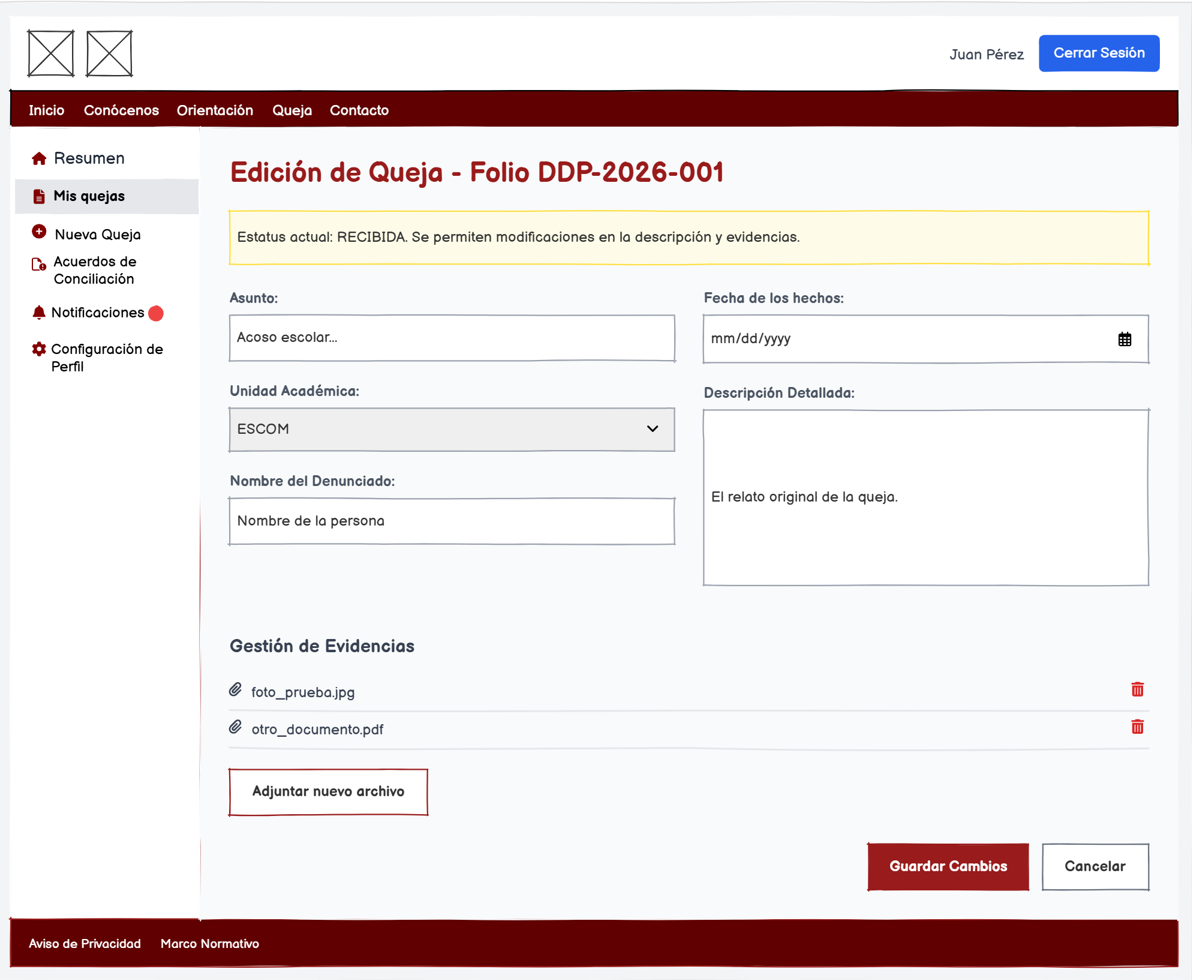
\includegraphics[width=0.80\textwidth, height=0.70\textheight, keepaspectratio]{imagenes/quejoso/Mockups/MQ-13_EditarQueja.png}
        \caption{Mockup MQ-13: Vista de Edición de Queja}
        \label{fig:mq13_editar_queja}
    \end{figure}
    
    % ---- MQ-14 ----
    \subsection{MQ-14: Ver Detalles de Queja}
    
    Interfaz de consulta de detalles de una queja. Despliega la información almacenada en un folio específico: datos del solicitante, cronología de estatus, narrativa de la queja y el repositorio de archivos adjuntos. Es una vista de solo lectura cuando el trámite ha avanzado a revisión.
    
    \begin{figure}[H]
        \centering
        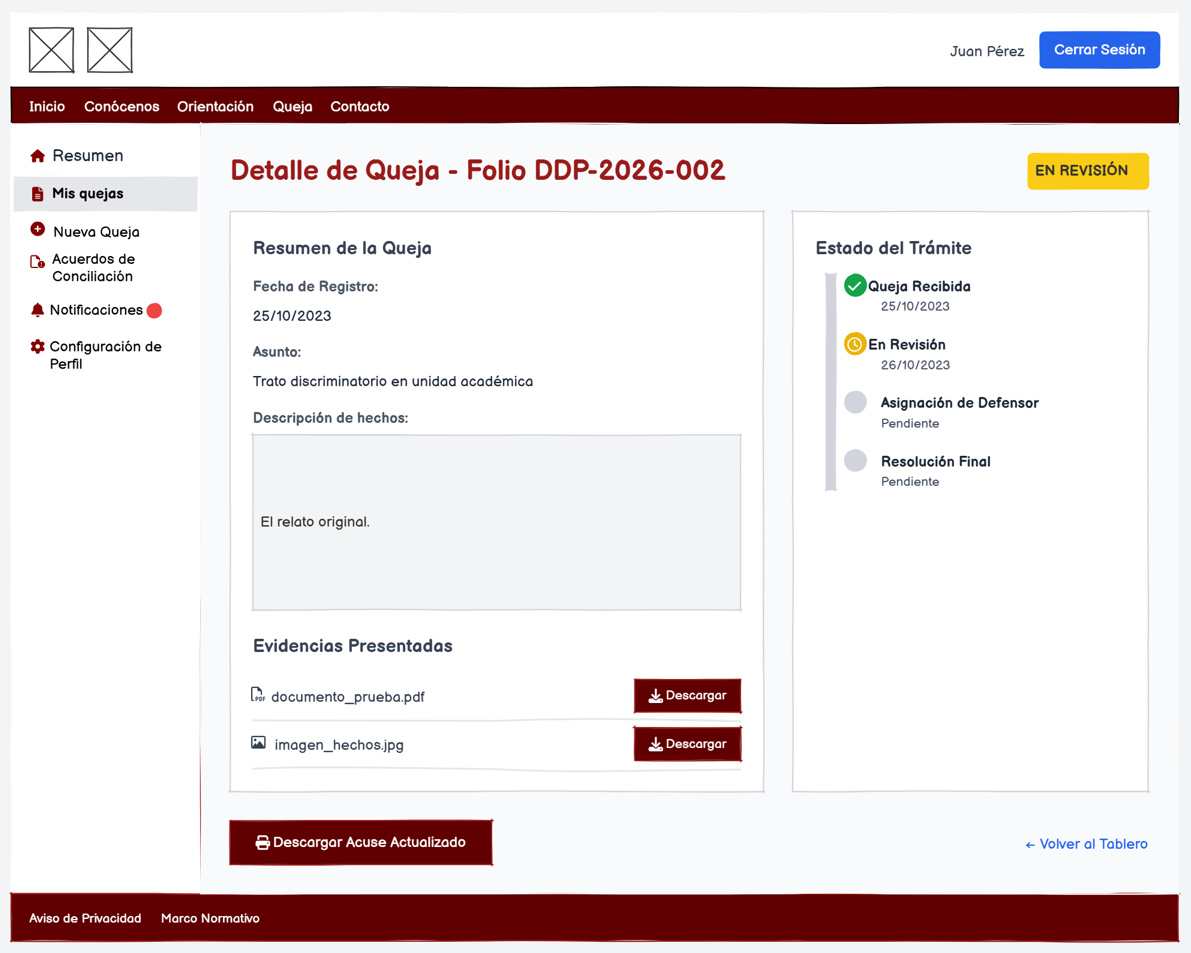
\includegraphics[width=0.80\textwidth, height=0.70\textheight, keepaspectratio]{imagenes/quejoso/Mockups/MQ-14_VerQueja.png}
        \caption{Mockup MQ-14: Vista de Detalle de Queja}
        \label{fig:mq14_ver_queja}
    \end{figure}
    
    % ---- MQ-15 ----
    \subsection{MQ-15: Historial de Quejas}
    
    Sección dedicada al un historial que presenta una tabla completa con todos los folios asociados al usuario. Incluye herramientas de filtrado avanzado por estatus y fecha, permitiendo al quejoso localizar expedientes históricos y descargar sus respectivos acuses de recibo.
    
    \begin{figure}[H]
        \centering
        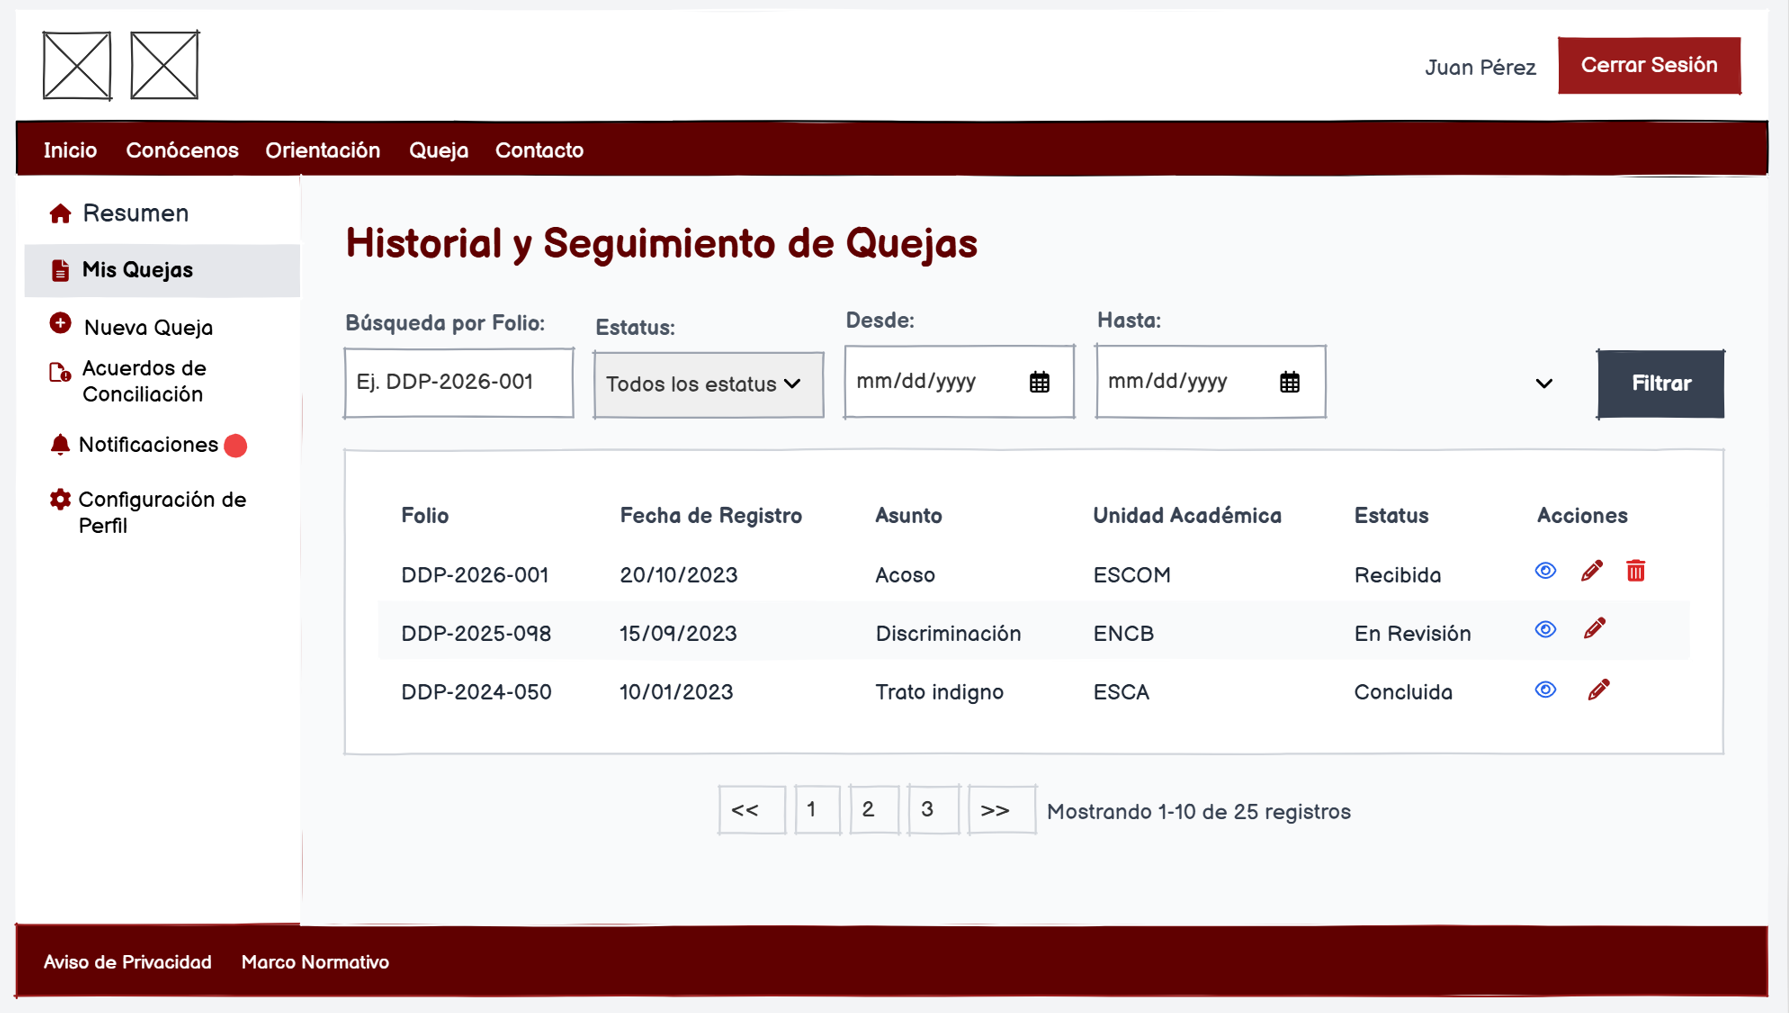
\includegraphics[width=0.80\textwidth, height=0.70\textheight, keepaspectratio]{imagenes/quejoso/Mockups/MQ-15_HistorialQuejas.png}
        \caption{Mockup MQ-15: Historial de Quejas del Usuario}
        \label{fig:mq15_historial_quejas}
    \end{figure}
    
    % ---- MQ-16 ----
    \subsection{MQ-16: Nueva Queja (Autenticado)}
    
    Formulario optimizado para levantar una nueva queja. A diferencia del registro público, esta interfaz recupera automáticamente los datos de perfil del usuario (nombre, correo, teléfono), permitiendo que el quejoso se enfoque únicamente en describir los nuevos hechos y adjuntar las evidencias correspondientes.
    
    \begin{figure}[H]
        \centering
        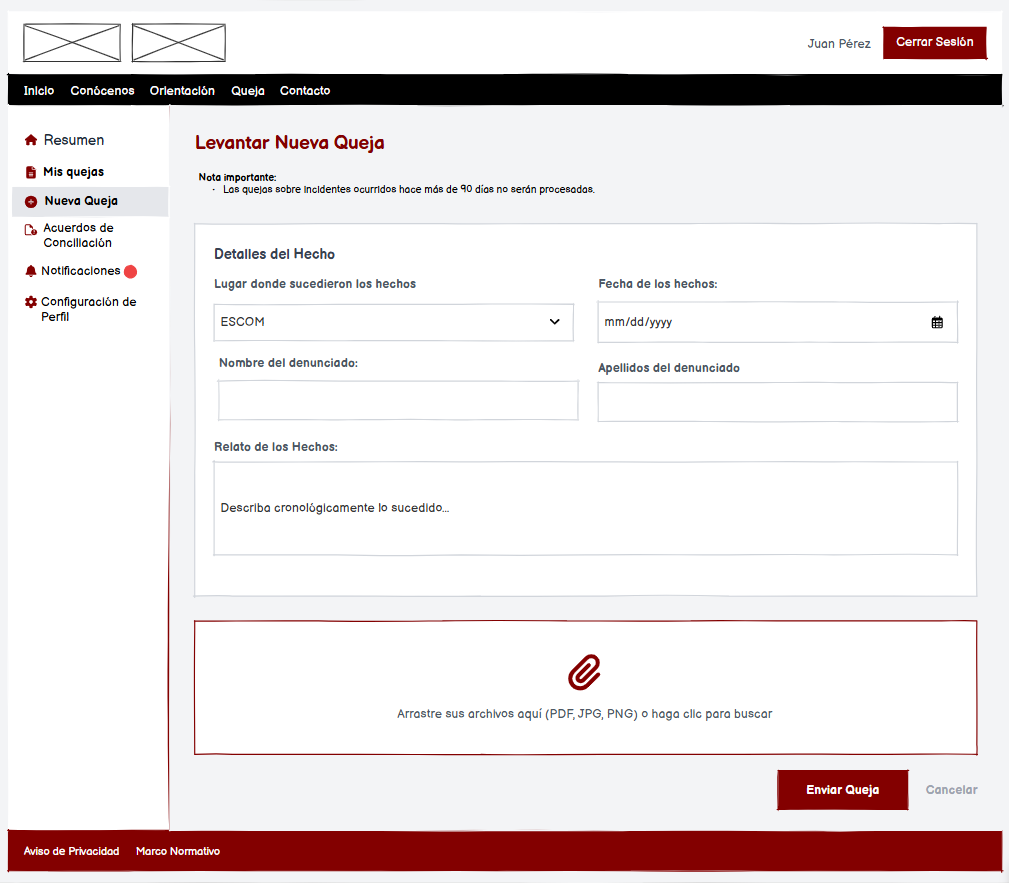
\includegraphics[width=0.80\textwidth, height=0.70\textheight, keepaspectratio]{imagenes/quejoso/Mockups/MQ-16_NuevaQueja.png}
        \caption{Mockup MQ-16: Formulario de Nueva Queja (Usuario Autenticado)}
        \label{fig:mq16_nueva_queja}
    \end{figure}
    
    % ---- MQ-17 ----
    \subsection{MQ-17: Folio de Cuenta}
    
    Vista de éxito tras registrar una nueva queja estando autenticado. Muestra el nuevo folio asignado y permite regresar de manera inmediata a la gestión de trámites, asegurando que el nuevo expediente aparezca actualizado en el historial del usuario.
    
    \begin{figure}[H]
        \centering
        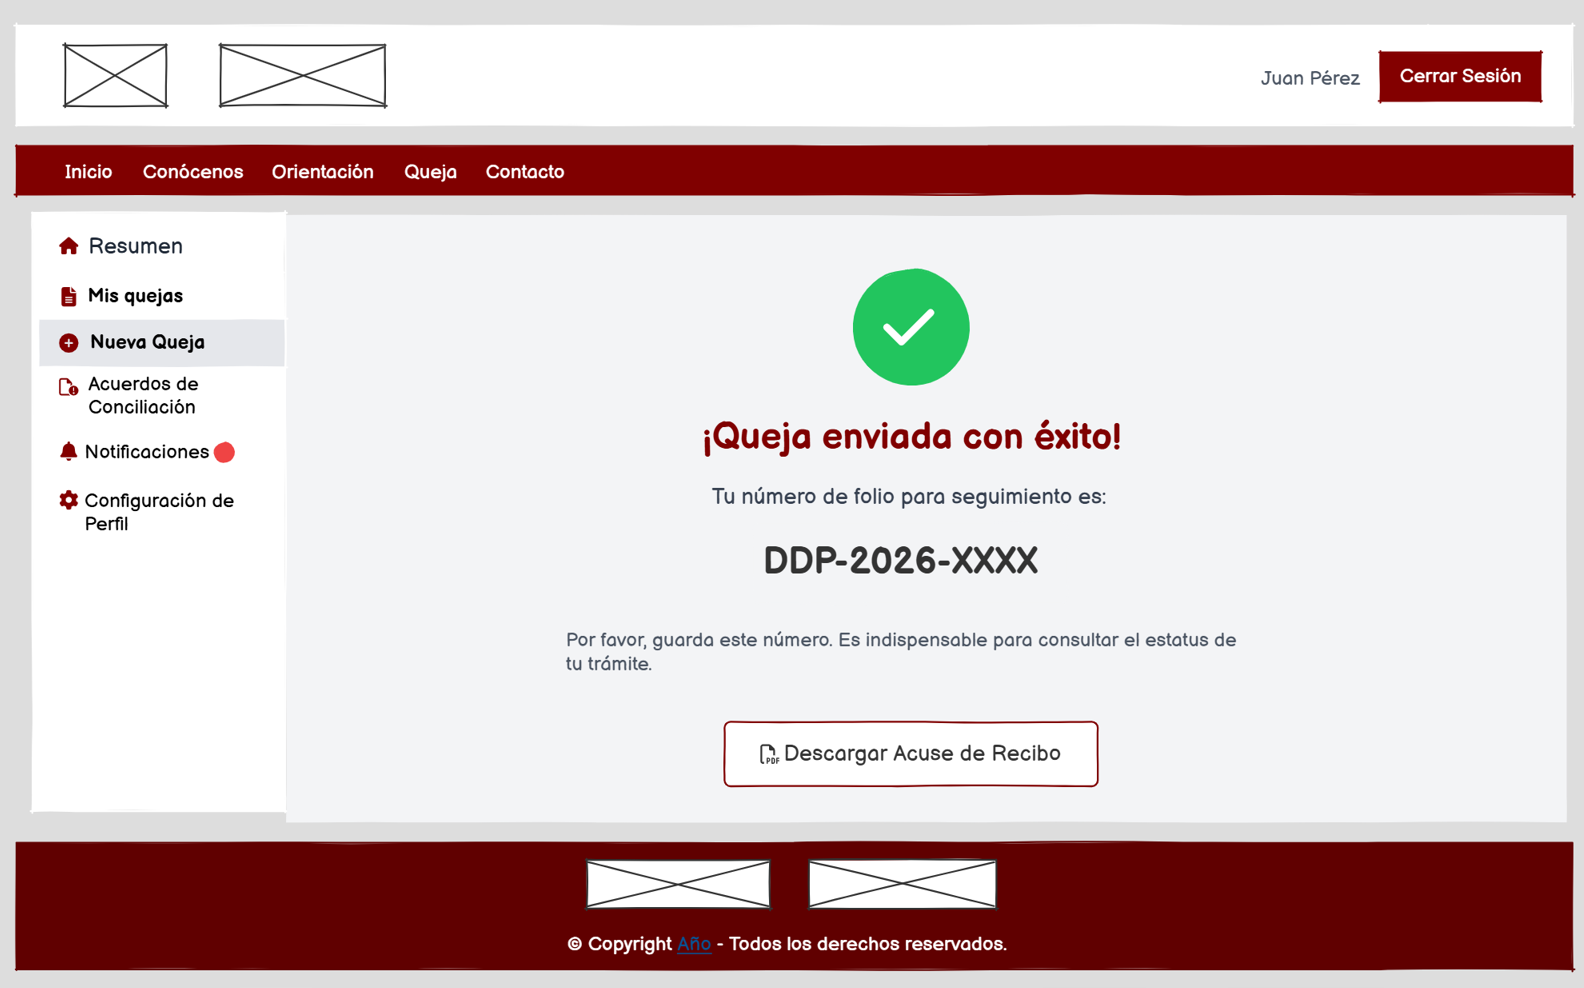
\includegraphics[width=0.80\textwidth, height=0.70\textheight, keepaspectratio]{imagenes/quejoso/Mockups/MQ-17_FolioCuenta.png}
        \caption{Mockup MQ-17: Confirmación de Folio en Cuenta Autenticada}
        \label{fig:mq17_folio_cuenta}
    \end{figure}
    
    % ---- MQ-18 ----
    \subsection{MQ-18: Acuerdos de Conciliación}
    
    Vista que agrupa los expedientes que han recibido una respuesta por parte del defensor. Permite al usuario identificar rápidamente cuáles de sus trámites tienen una propuesta pendiente de revisión, facilitando la transición hacia la resolución del conflicto.
    
    \begin{figure}[H]
        \centering
        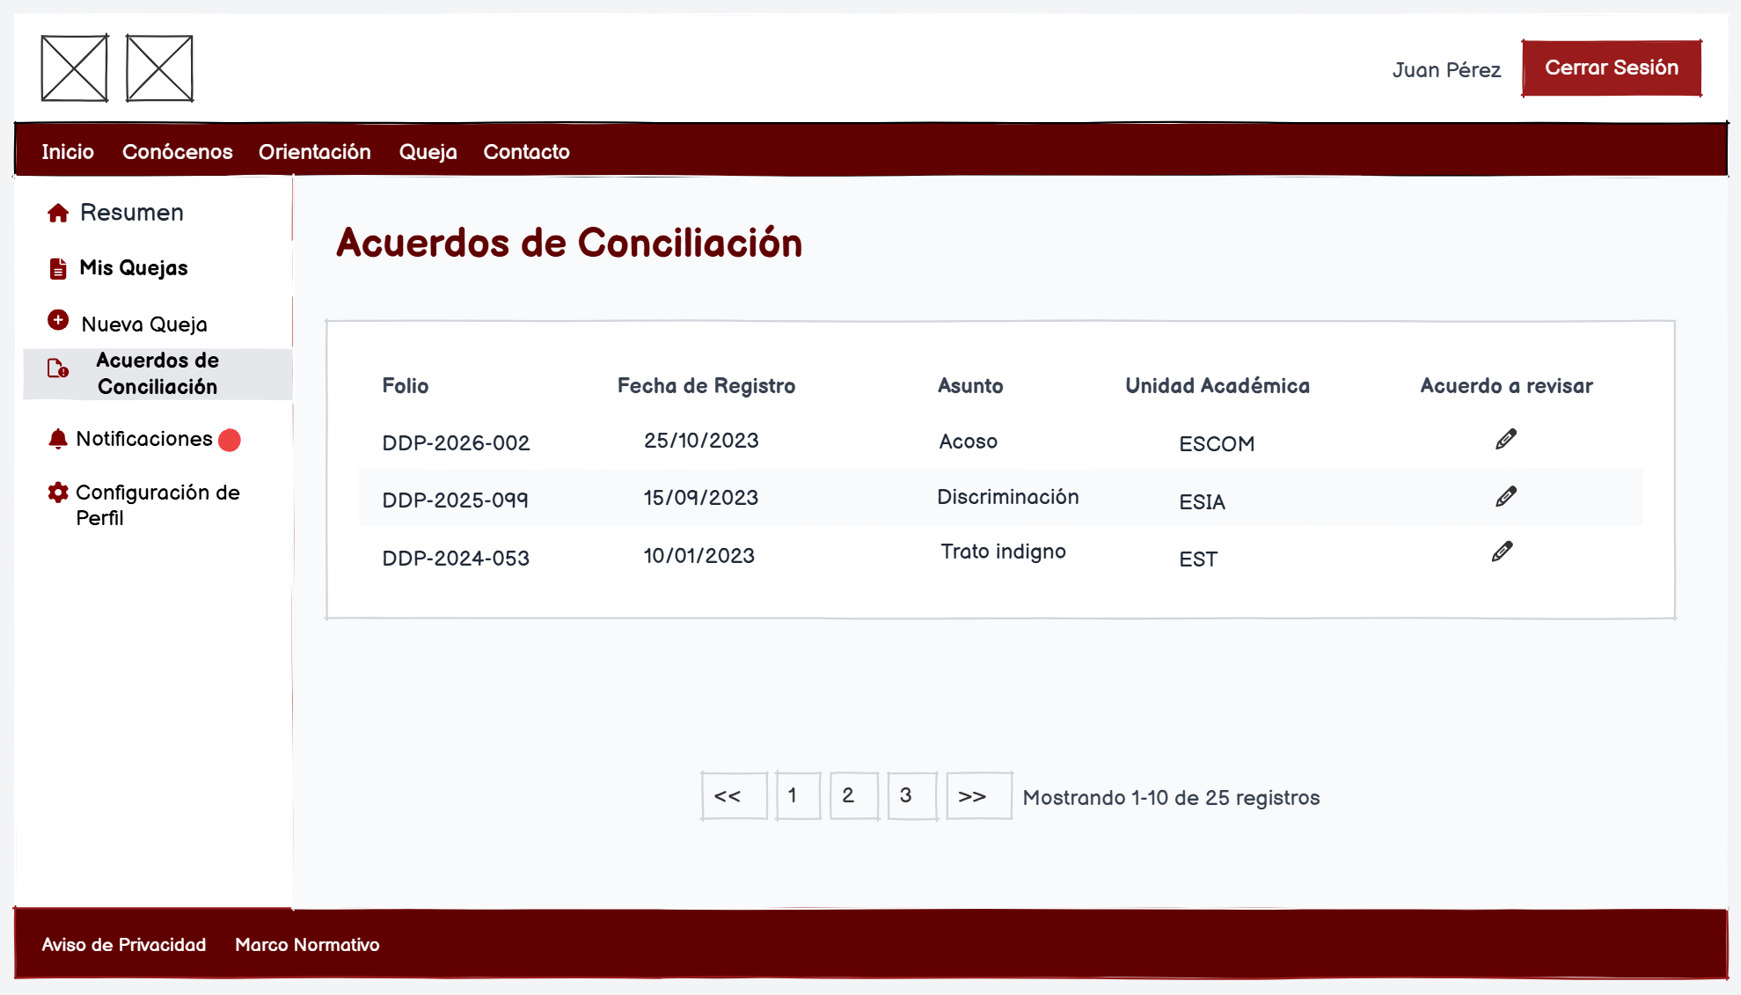
\includegraphics[width=0.80\textwidth, height=0.70\textheight, keepaspectratio]{imagenes/quejoso/Mockups/MQ-18_AcuerdosConciliacion.png}
        \caption{Mockup MQ-18: Vista de Acuerdos de Conciliación}
        \label{fig:mq18_acuerdos_conciliacion}
    \end{figure}
    
    % ---- MQ-19 ----
    \subsection{MQ-19: Propuesta de Conciliación}
    
    Pantalla para los procesos el proceso de aceptar o rechazar un acuerdo de conciliación. Presenta el texto de la solución propuesta por la Defensoría y habilita los controles vinculantes para que el quejoso pueda "Aceptar" o "Rechazar" la propuesta. En caso de rechazo, la interfaz solicita la justificación obligatoria.
    
    \begin{figure}[H]
        \centering
        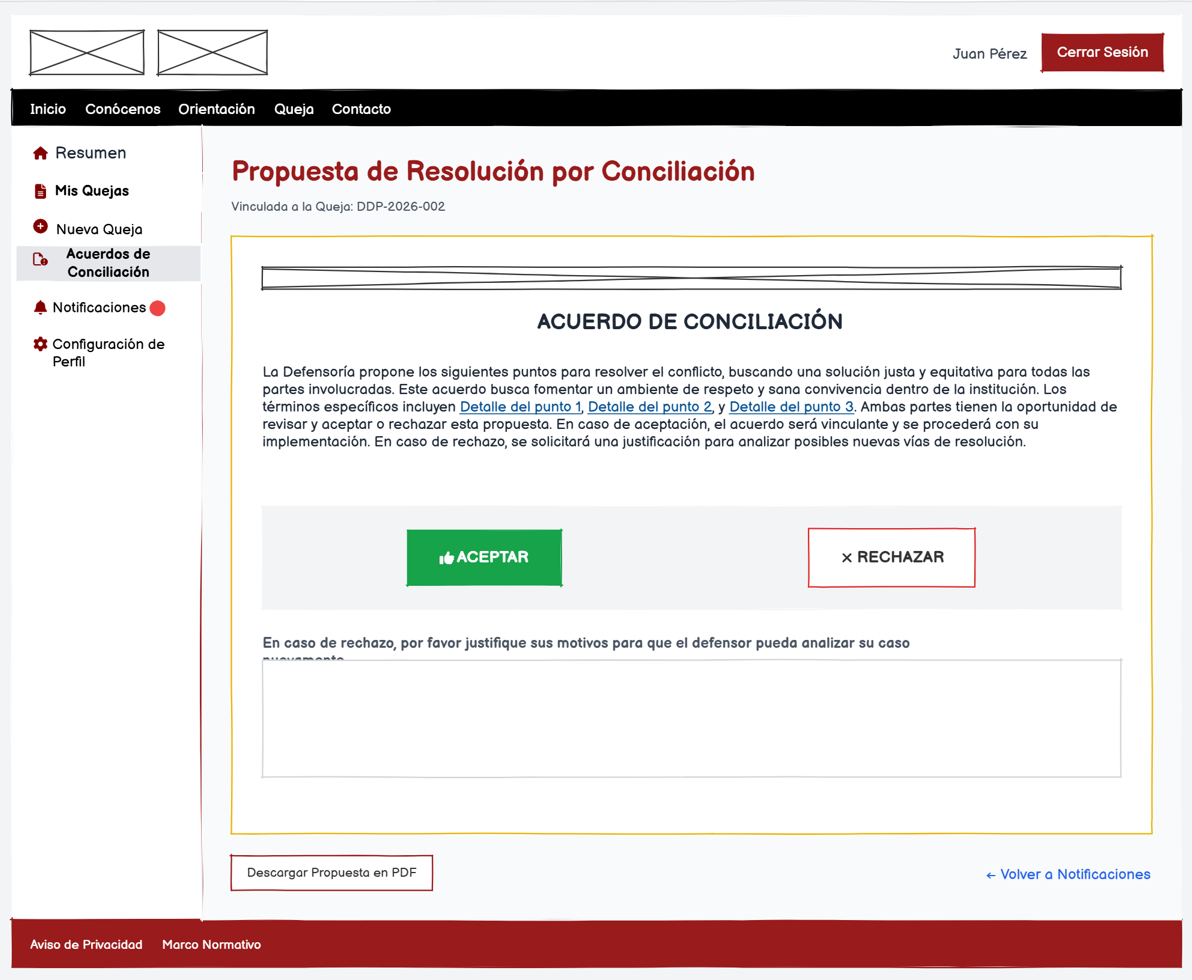
\includegraphics[width=0.80\textwidth, height=0.70\textheight, keepaspectratio]{imagenes/quejoso/Mockups/MQ-19_PropuestaConciliacion.png}
        \caption{Mockup MQ-19: Detalle de Propuesta de Conciliación}
        \label{fig:mq19_propuesta_conciliacion}
    \end{figure}
    
    % ---- MQ-20 ----
    \subsection{MQ-20: Notificaciones}
    
    Interfaz de alertas diseñada para mostrar una lista cronológica de eventos relevantes, como cambios de estatus en los expedientes o requerimientos de información adicional, permitiendo al quejoso mantenerse actualizado sobre el progreso administrativo de sus quejas.
    
    \begin{figure}[H]
        \centering
        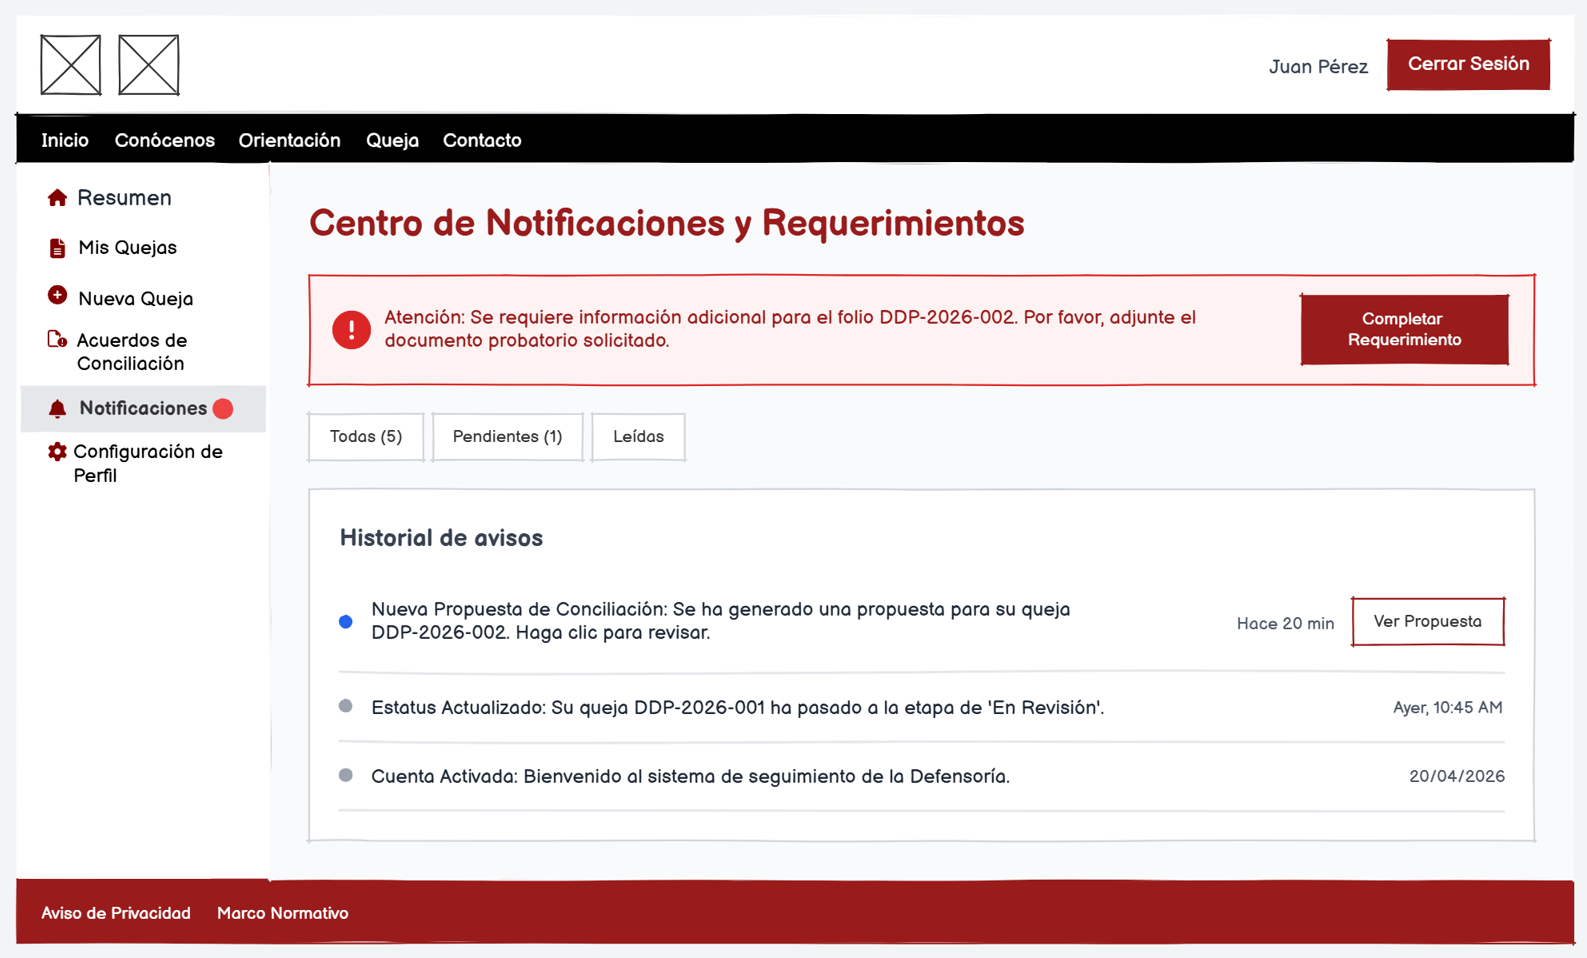
\includegraphics[width=0.80\textwidth, height=0.70\textheight, keepaspectratio]{imagenes/quejoso/Mockups/MQ-20_Notificaciones.png}
        \caption{Mockup MQ-20: Centro de Notificaciones}
        \label{fig:mq20_notificaciones}
    \end{figure}
    
    % ---- MQ-21 ----
    \subsection{MQ-21: Configuración de Perfil}
    
    Vista de perfil del quejoso autenticado. Muestra la información personal registrada en el sistema —nombre, correo, teléfono y datos del tutor si aplica— y permite editar los datos de contacto para mantenerlos actualizados durante el proceso de atención.
    
    \begin{figure}[H]
        \centering
        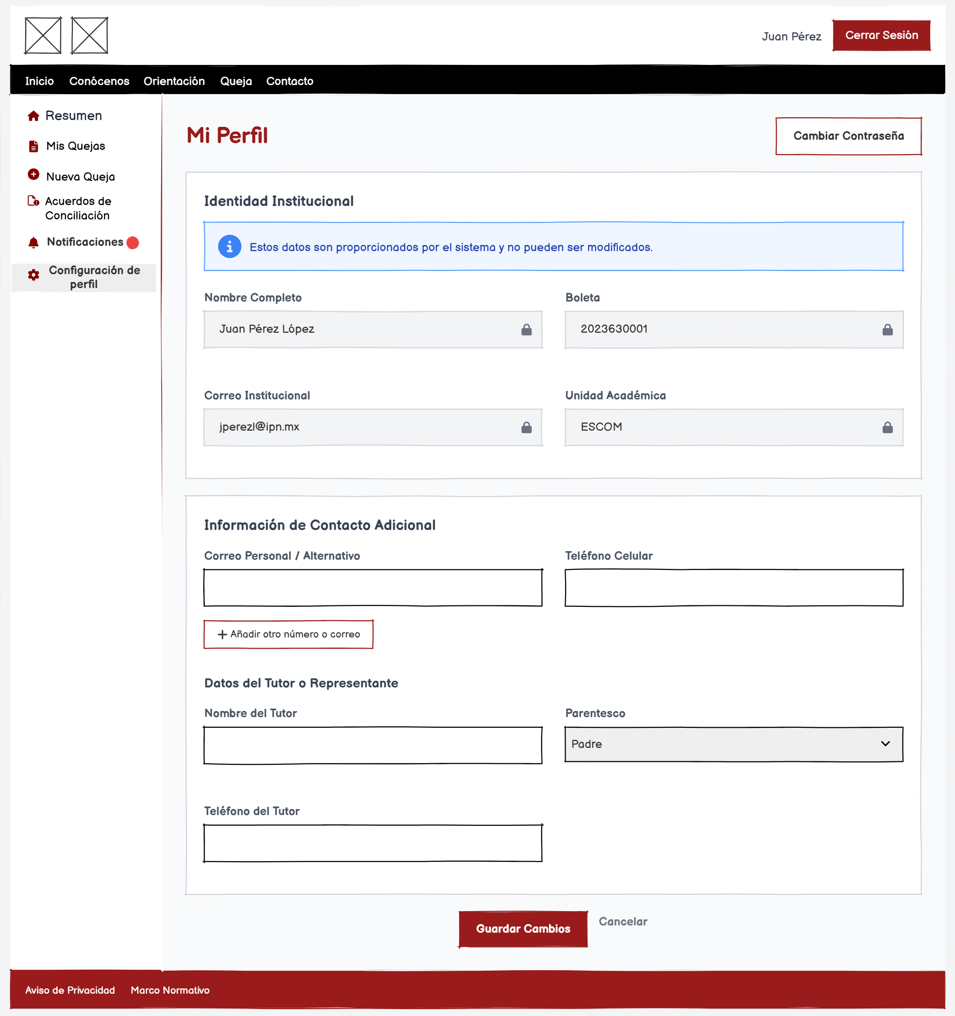
\includegraphics[width=0.80\textwidth, height=0.70\textheight, keepaspectratio]{imagenes/quejoso/Mockups/MQ-21_ConfiguracionPerfil.png}
        \caption{Mockup MQ-21: Configuración de Perfil del Quejoso}
        \label{fig:mq21_configuracion_perfil}
    \end{figure}
    
\section{Perfil: Administración y Defensoría}
Este perfil integra las herramientas de gestión interna de la plataforma. El acceso está restringido al personal de la Defensoría de los Derechos Politécnicos y se divide en cuatro departamentos operativos con facultades diferenciadas para garantizar la debida atención de los expedientes.

% --- VISTA ADMINISTRATIVA 01 ---
\begin{figure}[h]
\centering
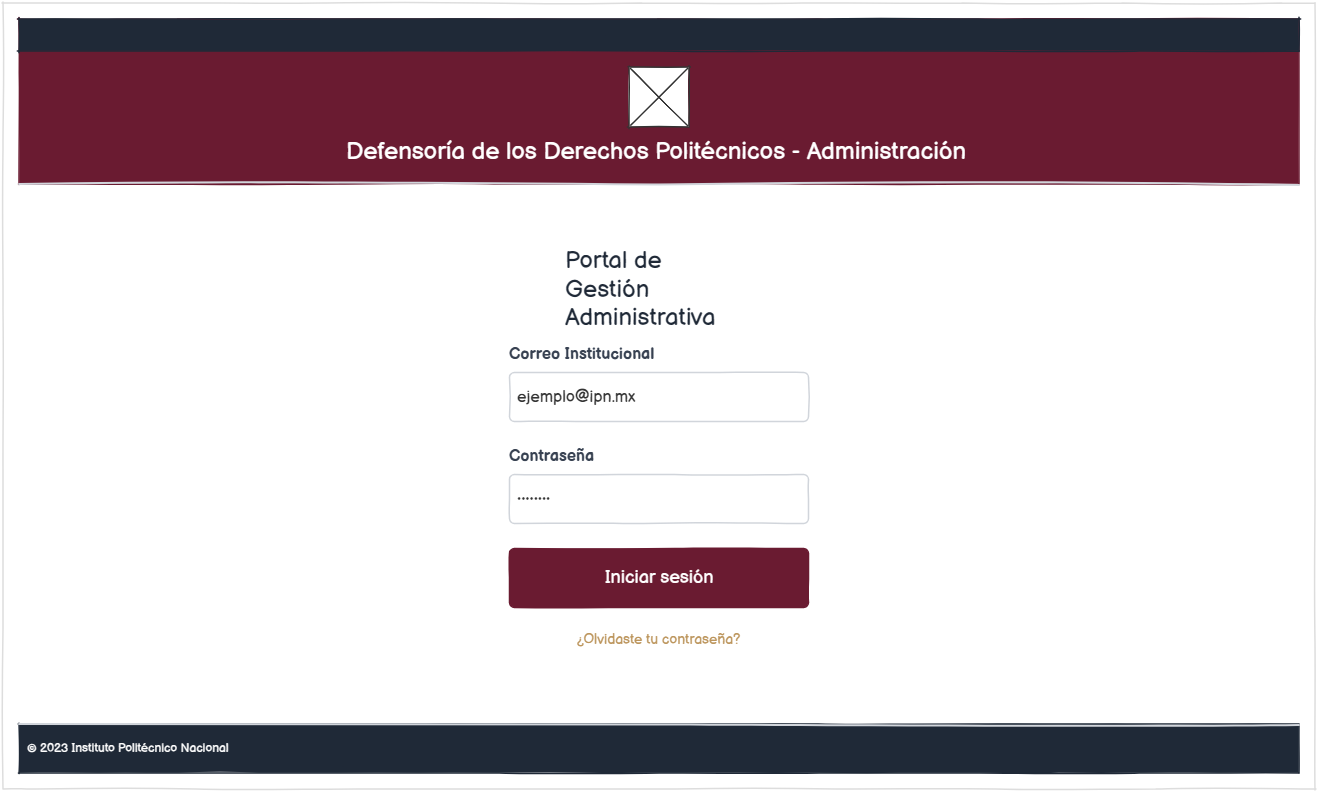
\includegraphics[width=0.65\textwidth]{imagenes/recepcion/InicioSesión_DDP.png}
\caption{MA-01: Portal de acceso al Sistema de Gestión Administrativa.}
\label{fig:ma01_login_adm}
\end{figure}

\noindent \textbf{Descripción de la interfaz (MA-01):} \
Esta interfaz representa el punto de acceso unificado para el personal de la Defensoría de los Derechos Politécnicos. A diferencia del portal ciudadano, esta vista está optimizada para la seguridad interna mediante un encabezado de administración que identifica claramente el módulo para evitar confusiones. El sistema presenta campos de credenciales vinculados al directorio institucional y un pie de página oficial que refuerza el carácter normativo del portal, permitiendo un acceso seguro y restringido a las funciones de gestión.


\clearpage

% --- VISTA ADMINISTRATIVA 02 ---
\begin{figure}[h]
\centering
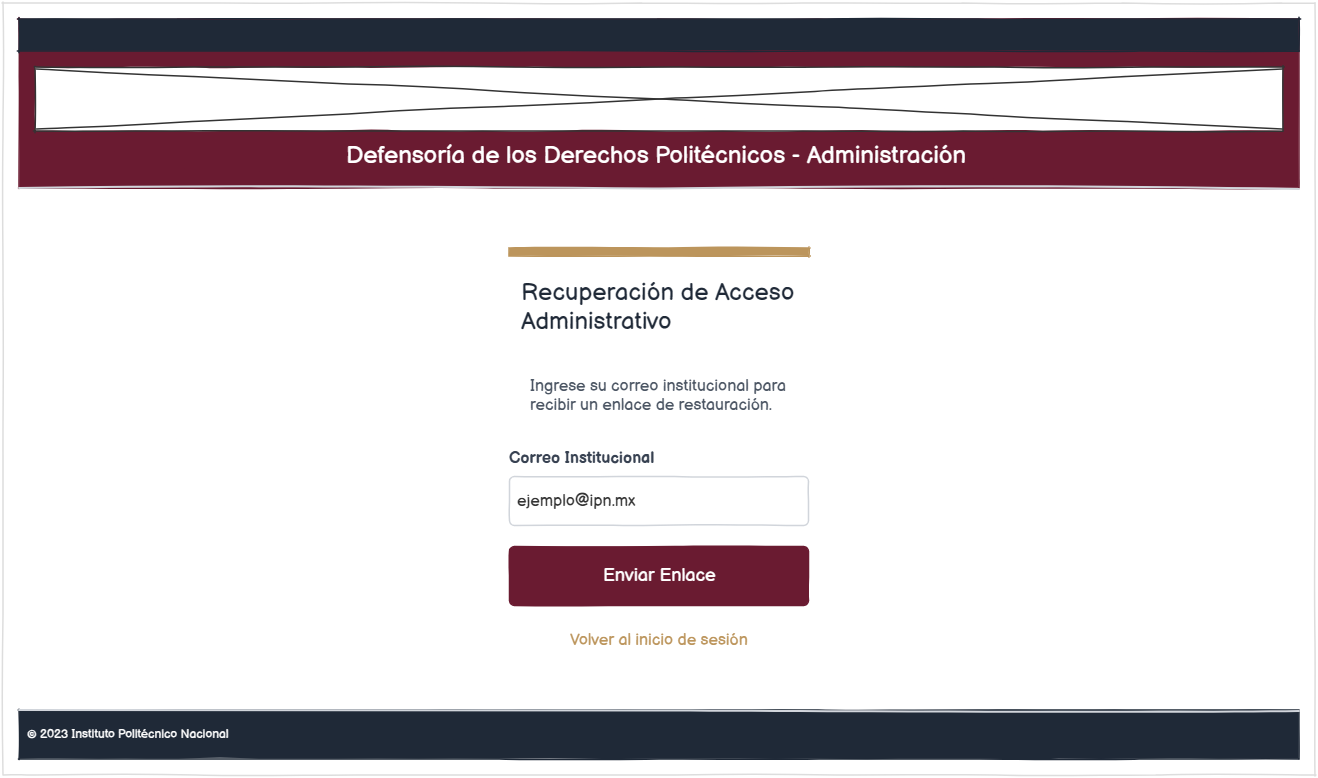
\includegraphics[width=0.65\textwidth]{imagenes/recepcion/RecuperaciónContraseñaDDP.png}
\caption{MA-02: Interfaz de recuperación de acceso para personal administrativo.}
\label{fig:ma02_recuperar_adm}
\end{figure}

\noindent \textbf{Descripción de la interfaz (MA-02):} \
Esta vista permite al personal de los cuatro departamentos restablecer sus credenciales de acceso de manera autónoma y segura. La validación institucional requiere exclusivamente el correo oficial para procesar la solicitud, asegurando que el enlace de restauración no sea desviado a cuentas externas. El flujo de recuperación cuenta con instrucciones directas y un control de navegación para volver al inicio de sesión, facilitando la recuperación del acceso sin comprometer la integridad del sistema administrativo.

\clearpage

\subsection{Departamento de Recepción}
Es el primer filtro del sistema, encargado de la validación inicial de los datos de entrada y la asignación preliminar de folios o turnos.

\begin{figure}[h]
\centering
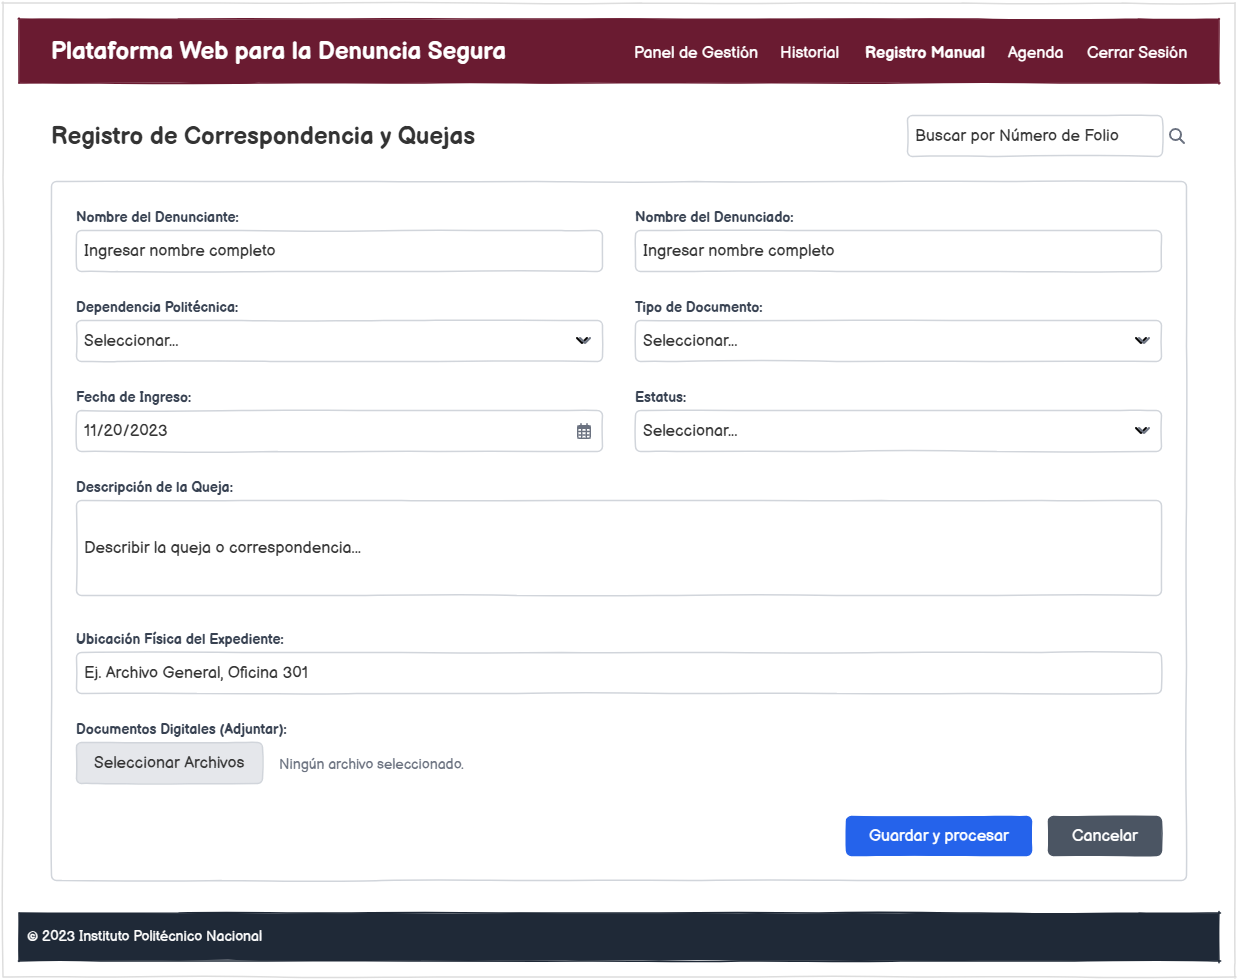
\includegraphics[width=0.65\textwidth]{imagenes/recepcion/RegistroManualQueja.png}
\caption{MA-03: Formulario de registro manual de correspondencia y quejas.}
\label{fig:ma03_registro_manual}
\end{figure}

\noindent \textbf{Descripción de la interfaz (MA-03):} \
Esta interfaz permite al personal administrativo registrar quejas o correspondencia recibida de manera presencial, facilitando la creación de un gemelo digital del expediente físico. La pantalla integra un buscador de folio para evitar duplicidad, campos para los datos de los sujetos involucrados y selectores para la clasificación administrativa y el estatus. Un elemento crítico es el campo especializado para registrar la ubicación del archivo físico, lo que garantiza la trazabilidad entre el papel original y el repositorio digital mediante la carga de evidencias escaneadas.


\clearpage

% --- VISTA 04: PANEL DE GESTIÓN ---
\begin{figure}[h]
\centering
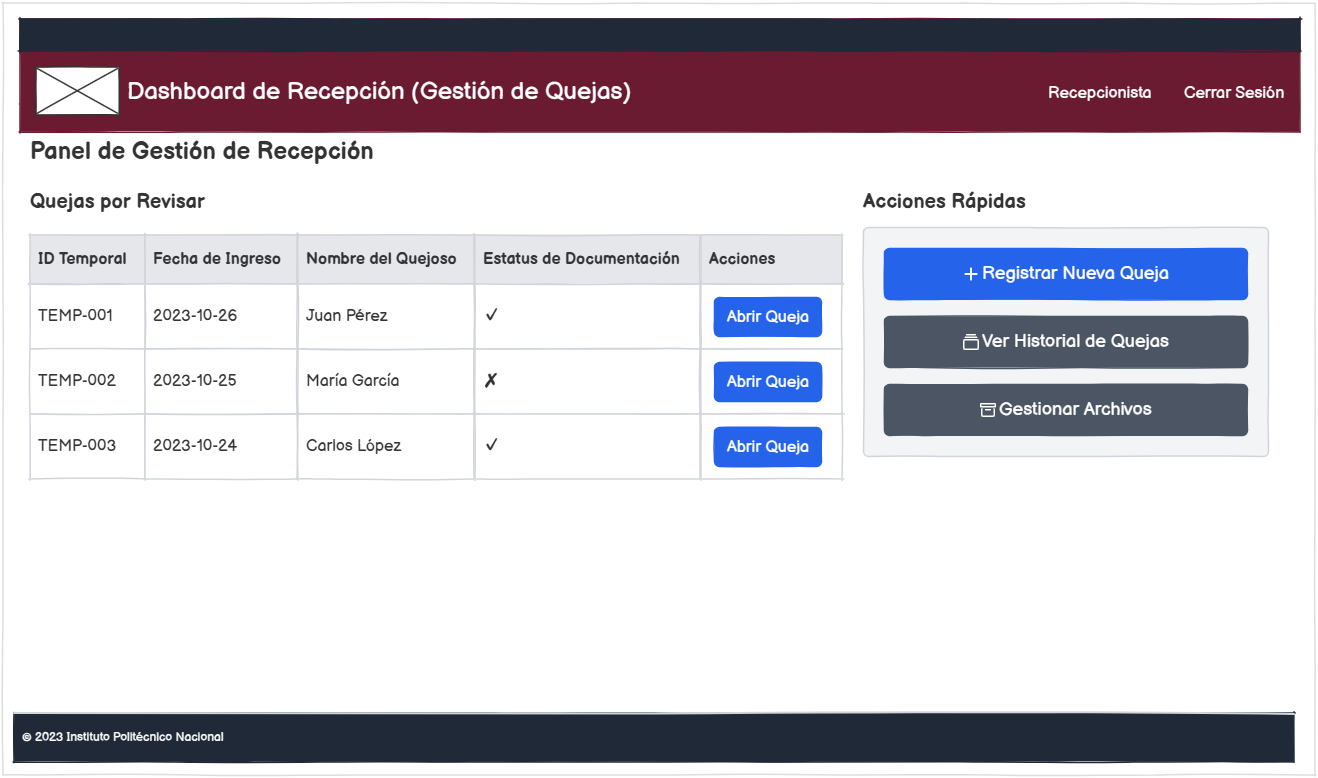
\includegraphics[width=0.65\textwidth]{imagenes/recepcion/PanelGestiónRecepción.png}
\caption{MA-04: Panel de gestión de recepción (Dashboard).}
\label{fig:ma04_dashboard_recepcion}
\end{figure}

\noindent \textbf{Descripción de la interfaz (MA-04):} \
Este tablero de control permite al personal de recepción monitorear las quejas entrantes de manera centralizada mediante una tabla operativa que utiliza identificadores temporales para registros pendientes de validación. La interfaz incluye indicadores visuales que señalan si un expediente cuenta con documentación completa, permitiendo el acceso directo al detalle de cada registro. Asimismo, un menú de acciones rápidas facilita tareas como el registro de nuevas quejas o la consulta del historial, manteniendo siempre visible el rol de recepcionista para asegurar la consistencia de los permisos.

\vspace{1cm}

% --- VISTA 05: VALIDACIÓN DE REQUISITOS ---
\begin{figure}[h]
\centering
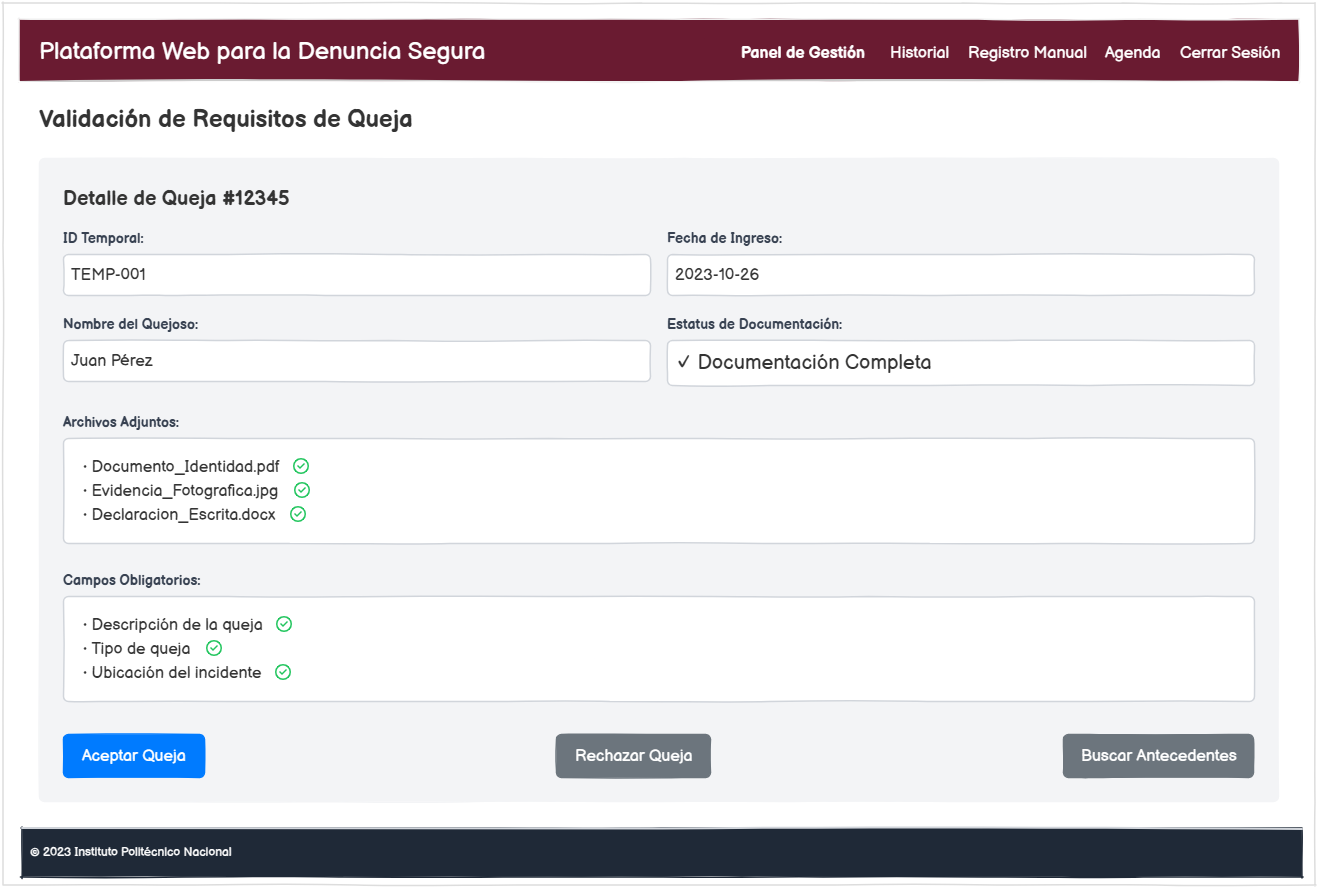
\includegraphics[width=0.65\textwidth]{imagenes/recepcion/ValidaciónRequisitosQueja.png}
\caption{MA-05: Módulo de validación de requisitos de queja.}
\label{fig:ma05_validacion_requisitos}
\end{figure}

\noindent \textbf{Descripción de la interfaz (MA-05):} \
Esta interfaz constituye el control de calidad del sistema, donde el personal asegura que cada solicitud cumpla con los estándares normativos. Presenta un resumen del expediente y un listado detallado de archivos adjuntos validados mediante iconos de verificación. El sistema obliga a la revisión de campos obligatorios como la descripción y la ubicación del incidente, concluyendo el proceso con botones de control que permiten aceptar la queja para su formalización, rechazarla por inconsistencias o realizar una búsqueda exhaustiva de antecedentes antes de su envío.

\vspace{1cm}

% --- VISTA 06: NOTIFICACIÓN DE RECHAZO ---
\begin{figure}[h]
\centering
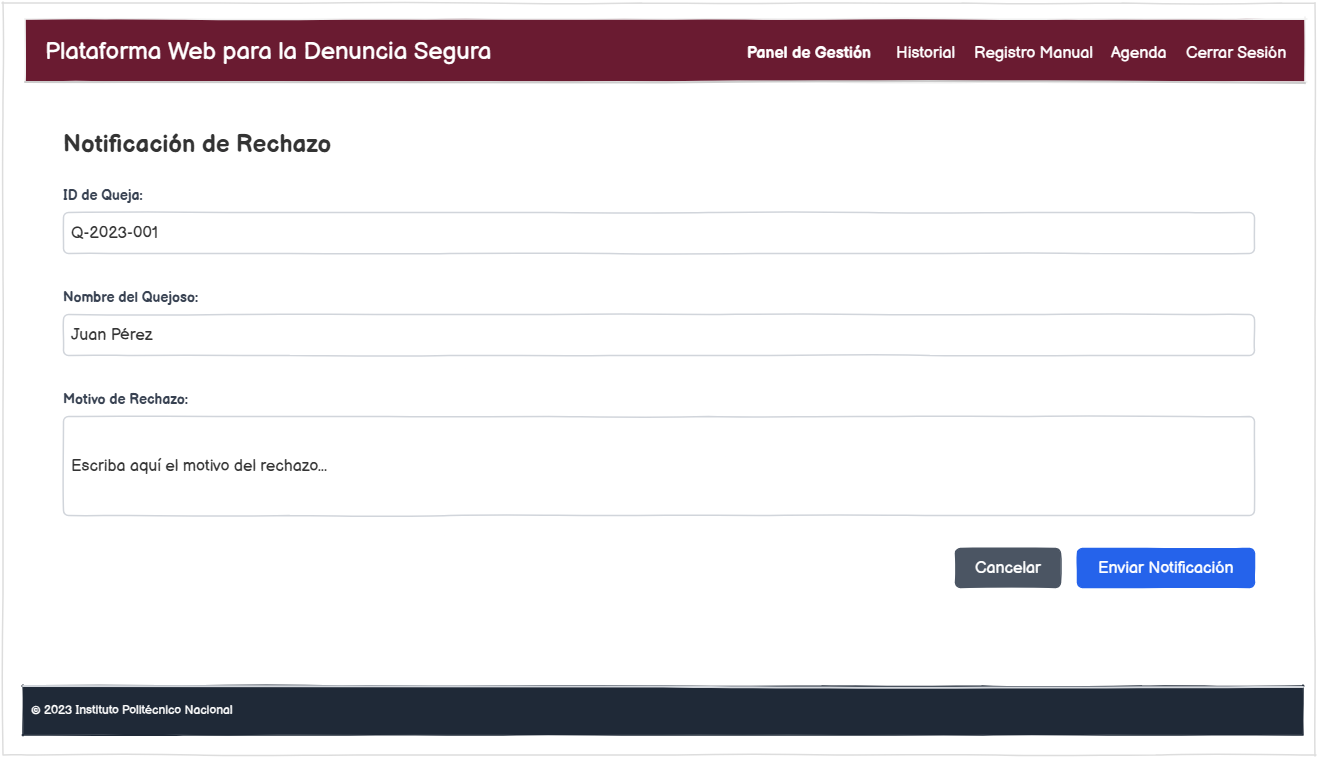
\includegraphics[width=0.65\textwidth]{imagenes/recepcion/NotificacionRechazo.png}
\caption{MA-06: Interfaz de notificación de rechazo por incumplimiento.}
\label{fig:ma06_notificacion_rechazo}
\end{figure}

\noindent \textbf{Descripción de la interfaz (MA-06):} \
Esta pantalla se activa al determinar que una solicitud no cumple con los requisitos mínimos, permitiendo informar al quejoso de manera formal sobre las deficiencias detectadas. La interfaz vincula automáticamente el ID del trámite y el nombre del usuario, ofreciendo un área de texto libre para que el administrativo redacte el motivo técnico o jurídico del rechazo. Una vez procesada la notificación, el sistema dispara un correo automático, permitiendo al personal retornar a sus labores mediante un menú de navegación persistente que conecta con la agenda e historial.

\vspace{1cm}

% --- VISTA 07: ANTECEDENTES Y CANALIZACIÓN ---
\begin{figure}[h]
\centering
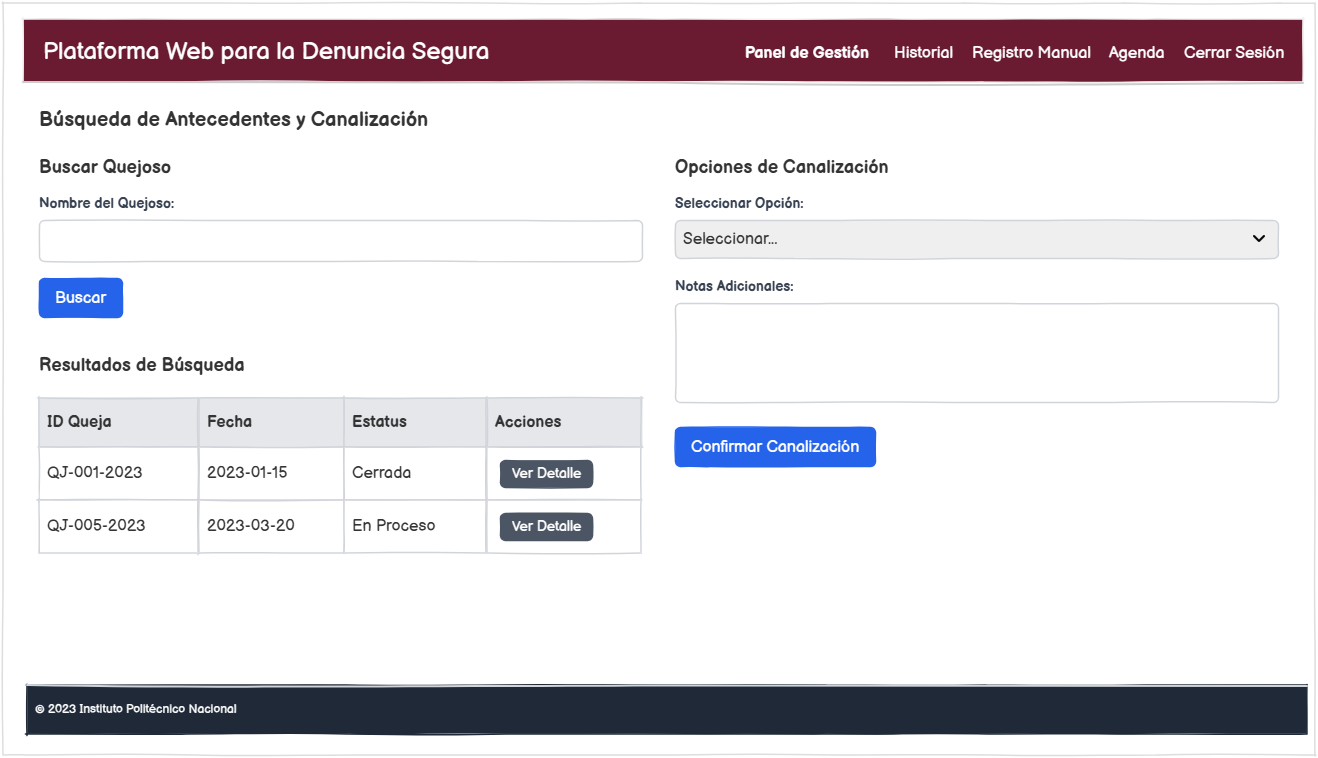
\includegraphics[width=0.65\textwidth]{imagenes/recepcion/BuesquedaAntecedentesCanalizacion.png}
\caption{MA-07: Módulo de búsqueda de antecedentes y canalización interna.}
\label{fig:ma07_canalizacion}
\end{figure}

\noindent \textbf{Descripción de la interfaz (MA-07):} \
Esta pantalla representa el último paso operativo en el área de Recepción, funcionando como motor de búsqueda y herramienta de traslado de expedientes. El sistema permite identificar procesos previos del quejoso para evitar duplicidades, mostrando una tabla de resultados con el historial de trámites anteriores. Para finalizar, el administrativo utiliza el panel de canalización para seleccionar el departamento de destino, agregando notas adicionales que orienten al siguiente analista antes de confirmar el envío y actualizar el estatus global del trámite.

\subsection{Departamento de Primer Contacto}
Este departamento se encarga de la atención personalizada al quejoso. Su función principal es realizar la entrevista inicial, analizar la naturaleza de la queja y determinar si el asunto es competencia de la Defensoría o si debe ser orientado a otra instancia.

% --- VISTA 08: BANDEJA DE ANÁLISIS ---
\begin{figure}[h]
\centering
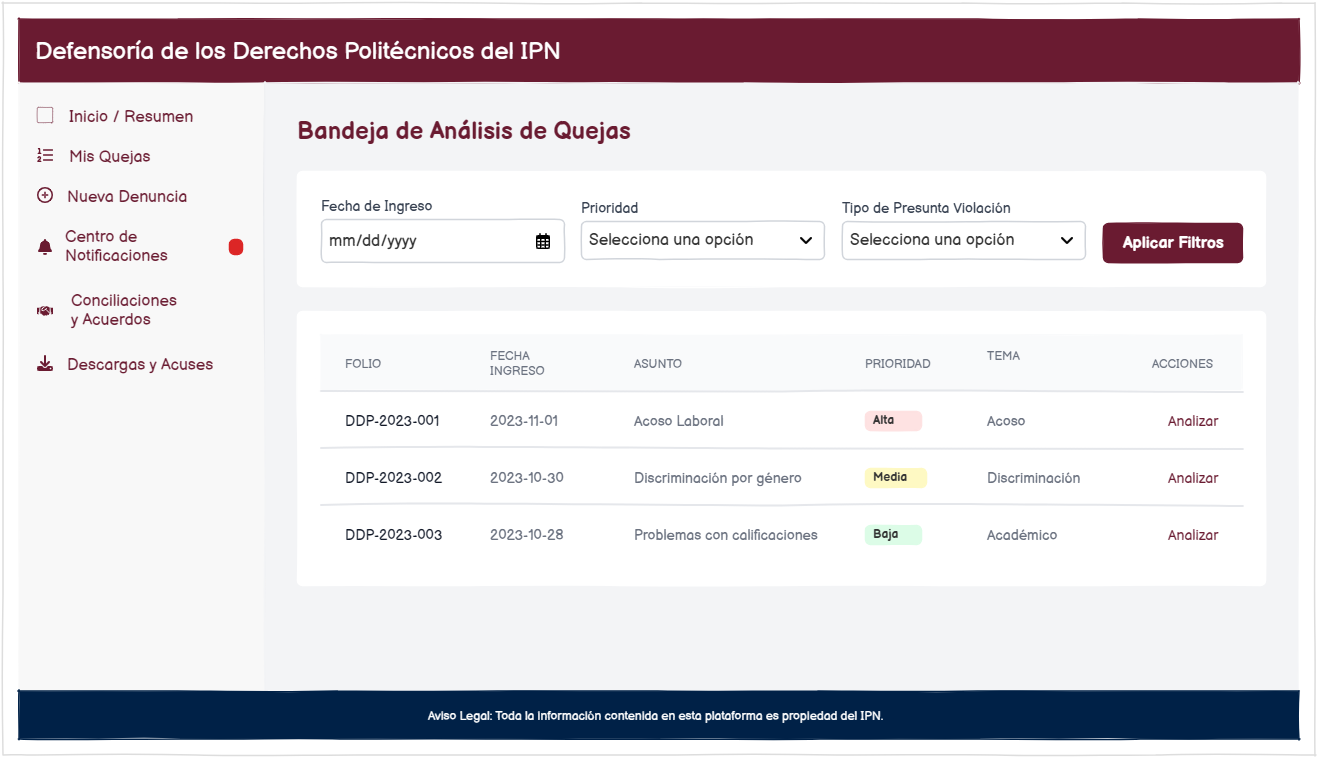
\includegraphics[width=0.65\textwidth]{imagenes/primercontacto/DashboardoAnalisisQuejas.png}
\caption{MA-08: Bandeja de análisis de quejas para Primer Contacto.}
\label{fig:ma08_analisis_dashboard}
\end{figure}

\noindent \textbf{Descripción de la interfaz (MA-08):} \
Esta interfaz constituye la herramienta principal del abogado o analista de Primer Contacto, diseñada para organizar de manera eficiente las quejas canalizadas desde el área de Recepción. La pantalla integra un módulo de filtrado avanzado que permite segmentar la carga de trabajo por fecha, prioridad y tipo de violación, facilitando la identificación de casos urgentes. A través de una tabla de gestión operativa, el personal puede visualizar los folios oficiales y los temas asignados, utilizando un sistema visual de etiquetas de colores para jerarquizar los hechos reportados. Finalmente, el control de análisis permite al funcionario acceder al detalle del expediente para iniciar formalmente la calificación jurídica.

\vspace{1cm}

\begin{figure}[h]
\centering
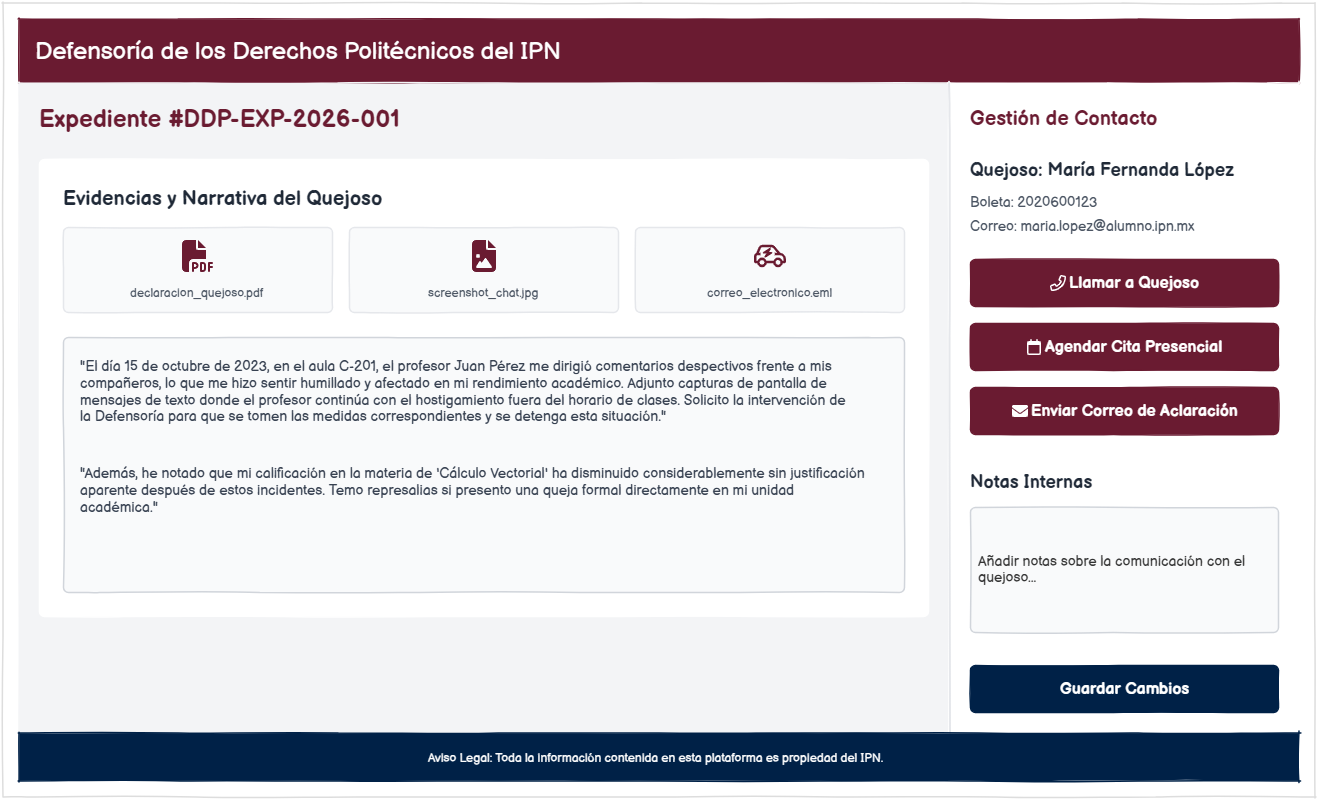
\includegraphics[width=0.65\textwidth]{imagenes/primercontacto/AnalisisExpediente.png}
\caption{MA-09: Interfaz de estudio de narrativa y evidencias.}
\label{fig:ma09_analisis_expediente}
\end{figure}

\noindent \textbf{Descripción de la interfaz (MQ-09):} \
Esta pantalla centraliza toda la información aportada por el quejoso para facilitar una evaluación legal exhaustiva por parte del analista. La interfaz dispone de un visor de evidencias con iconos diferenciados por formato, permitiendo una rápida revisión de los archivos adjuntos, junto a un área dedicada a la narrativa de los hechos para identificar presuntas violaciones de derechos. Además, se integra un panel de gestión de contacto con herramientas de comunicación inmediata para agendar citas o solicitar aclaraciones, complementado con una bitácora de notas internas donde el analista puede registrar observaciones técnicas que aseguren la continuidad del caso.

\clearpage


% --- VISTA 10: AGENDAR CITAS ---
\begin{figure}[h]
\centering
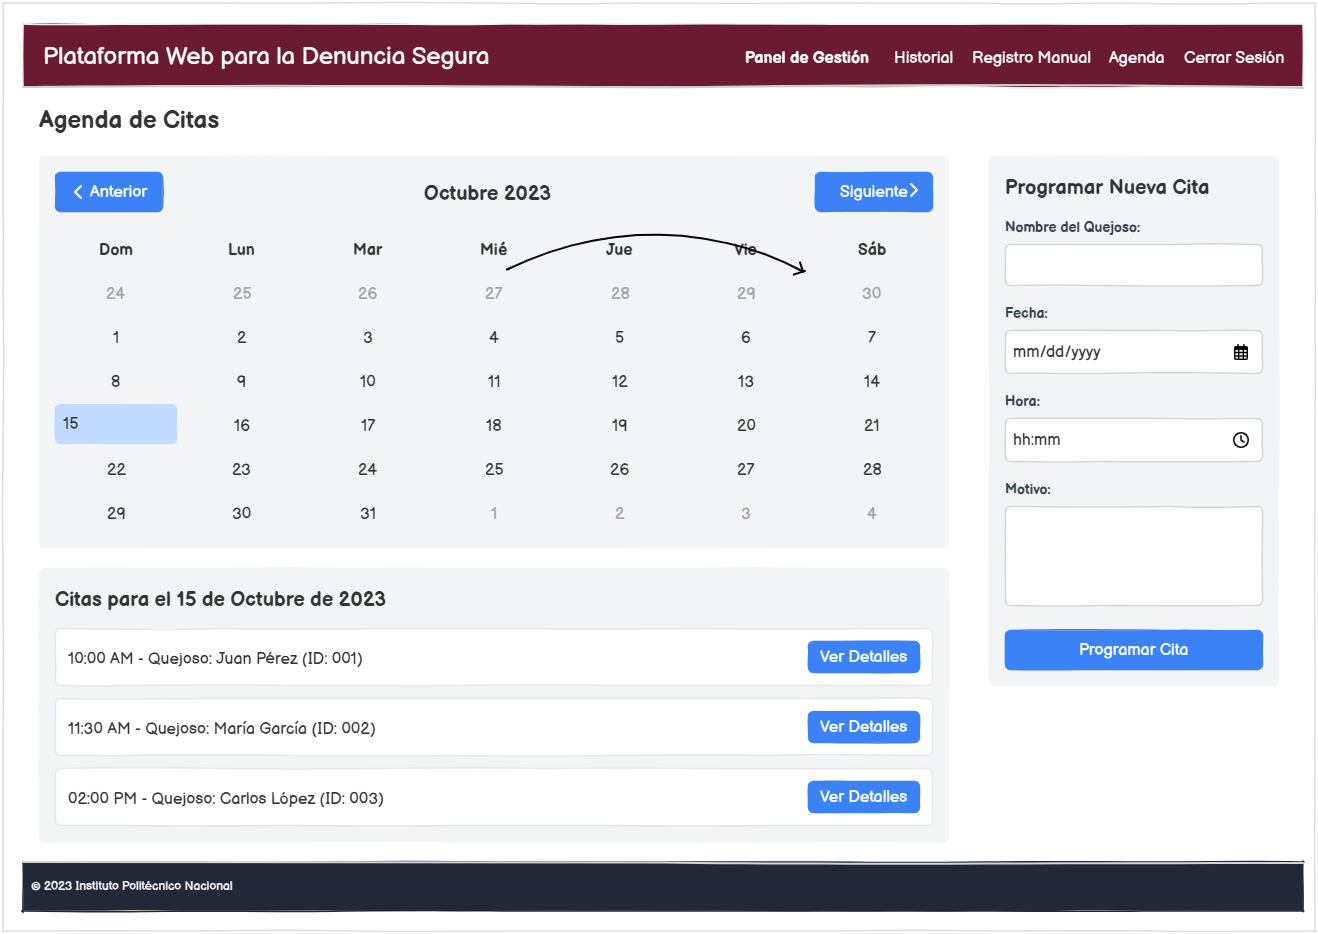
\includegraphics[width=0.65\textwidth]{imagenes/primercontacto/AgendarCitas.png}
\caption{MA-10: Módulo de agenda institucional para entrevistas de calificación.}
\label{fig:ma10_agenda_citas}
\end{figure}

\noindent \textbf{Descripción de la interfaz (MA-10):} \
Esta interfaz es fundamental para gestionar la interacción directa entre el analista y el quejoso, permitiendo organizar las diligencias necesarias para profundizar en los hechos. Presenta un calendario de disponibilidad dinámico que ayuda a evitar el traslape de horarios y optimiza el uso de las salas de entrevista, junto a un formulario lateral para capturar los detalles de cada reunión. El sistema vincula automáticamente al quejoso con una fecha y modalidad específica, manteniendo una lista de próximas entrevistas para la preparación previa del expediente. Al confirmar la cita, el estatus del trámite se actualiza automáticamente, notificando al usuario a través del portal correspondiente.

\clearpage


\begin{figure}[h]
\centering
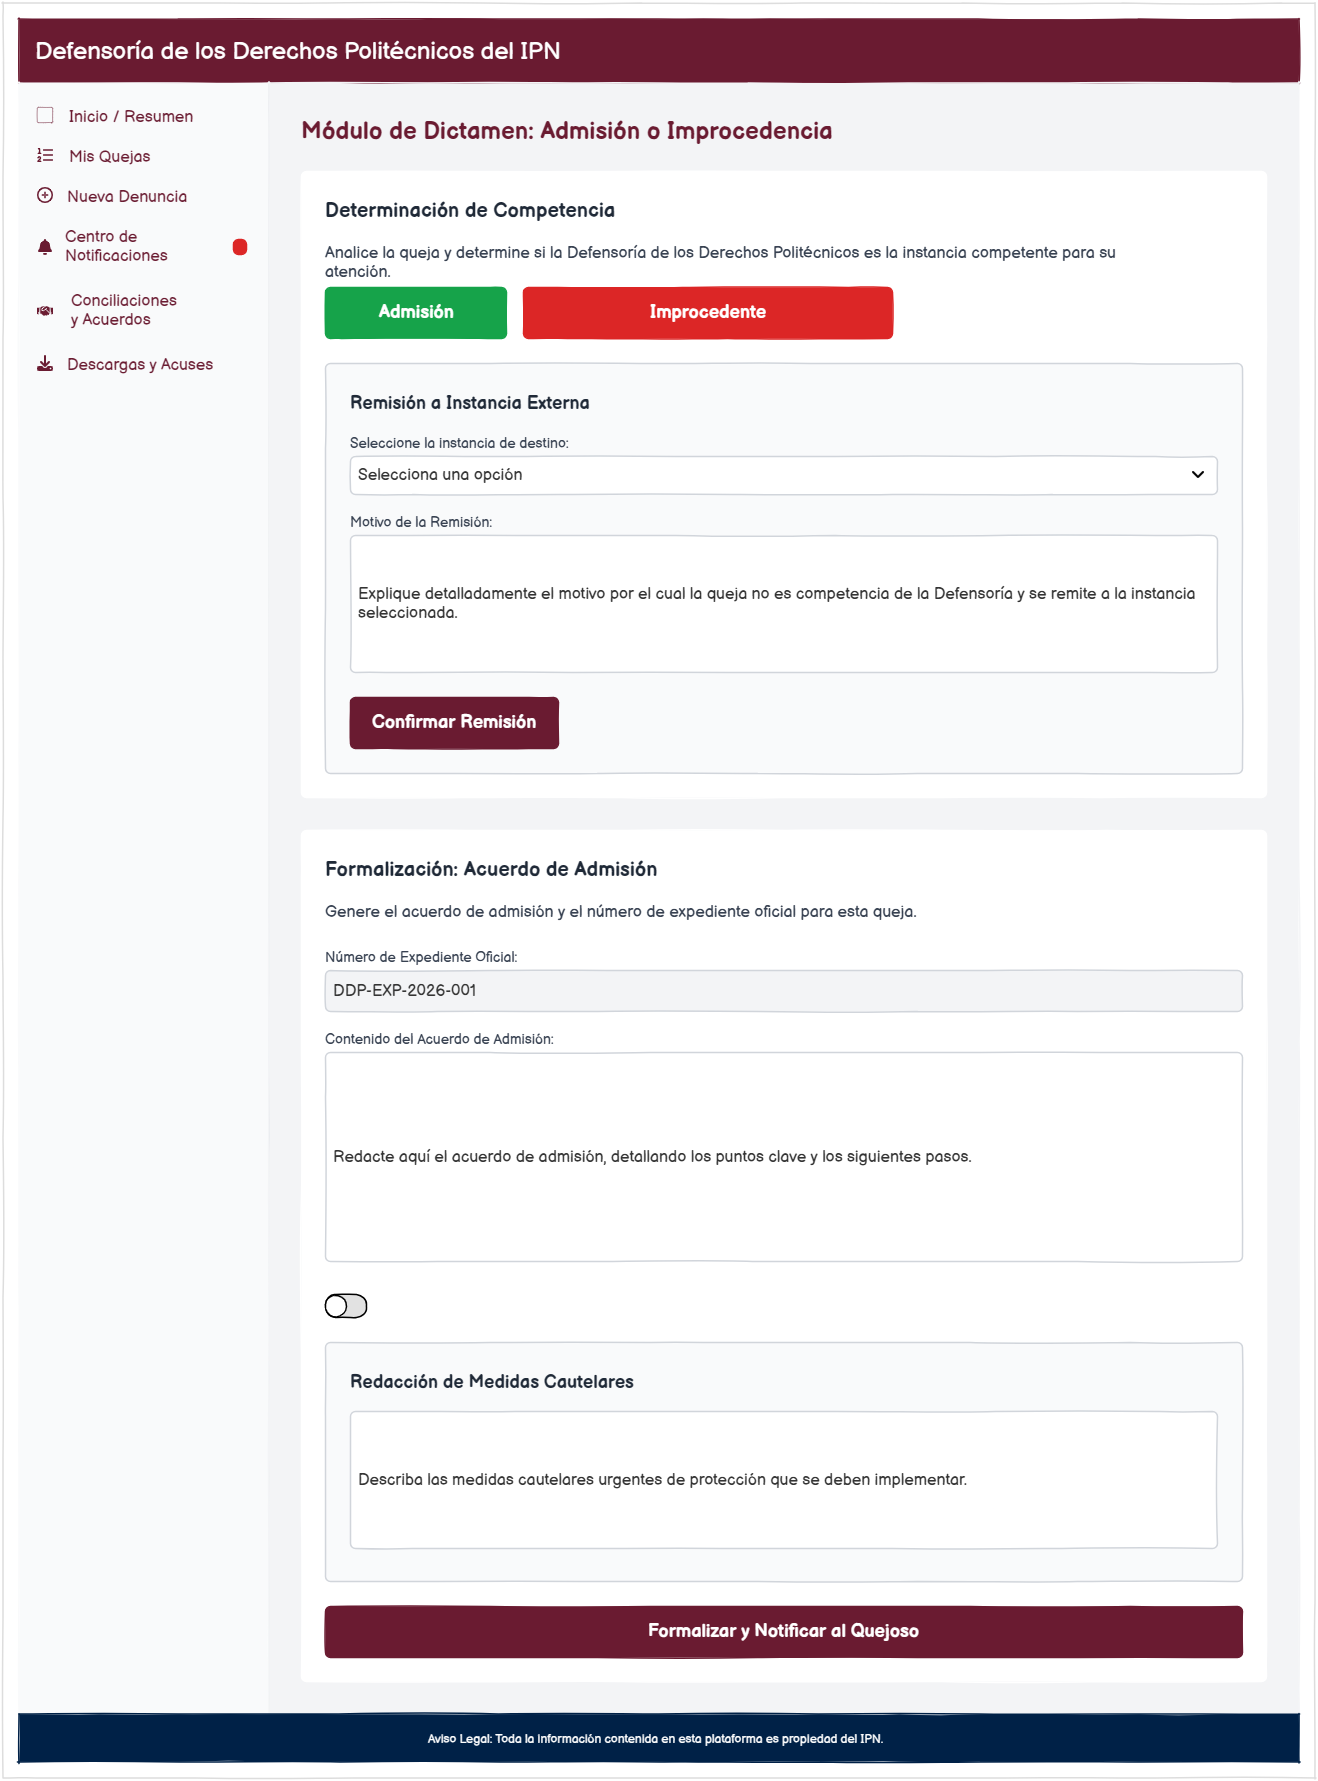
\includegraphics[width=0.65\textwidth]{imagenes/primercontacto/DictamenCompetencia}
\caption{MA-11: Módulo de dictamen de admisión o improcedencia.}
\label{fig:ma11_dictamen_competencia}
\end{figure}

\noindent \textbf{Descripción de la interfaz (MA-11):} \
Esta es la pantalla de resolución técnica donde se decide formalmente el curso legal de la queja presentada. El sistema ofrece botones de selección de alto contraste para definir la procedencia del caso, habilitando secciones específicas según la decisión tomada, ya sea para redactar los motivos legales de una improcedencia y su remisión externa, o para generar el número de expediente oficial en caso de admisión. La interfaz incluye también un control para la redacción de medidas cautelares urgentes en situaciones que requieran protección inmediata del quejoso. Una vez procesado el dictamen, el sistema formaliza el acto jurídico y prepara la notificación automática para el usuario.


\clearpage

% --- VISTA 12: FINALIZACIÓN Y NOTIFICACIÓN ---
\begin{figure}[h]
\centering
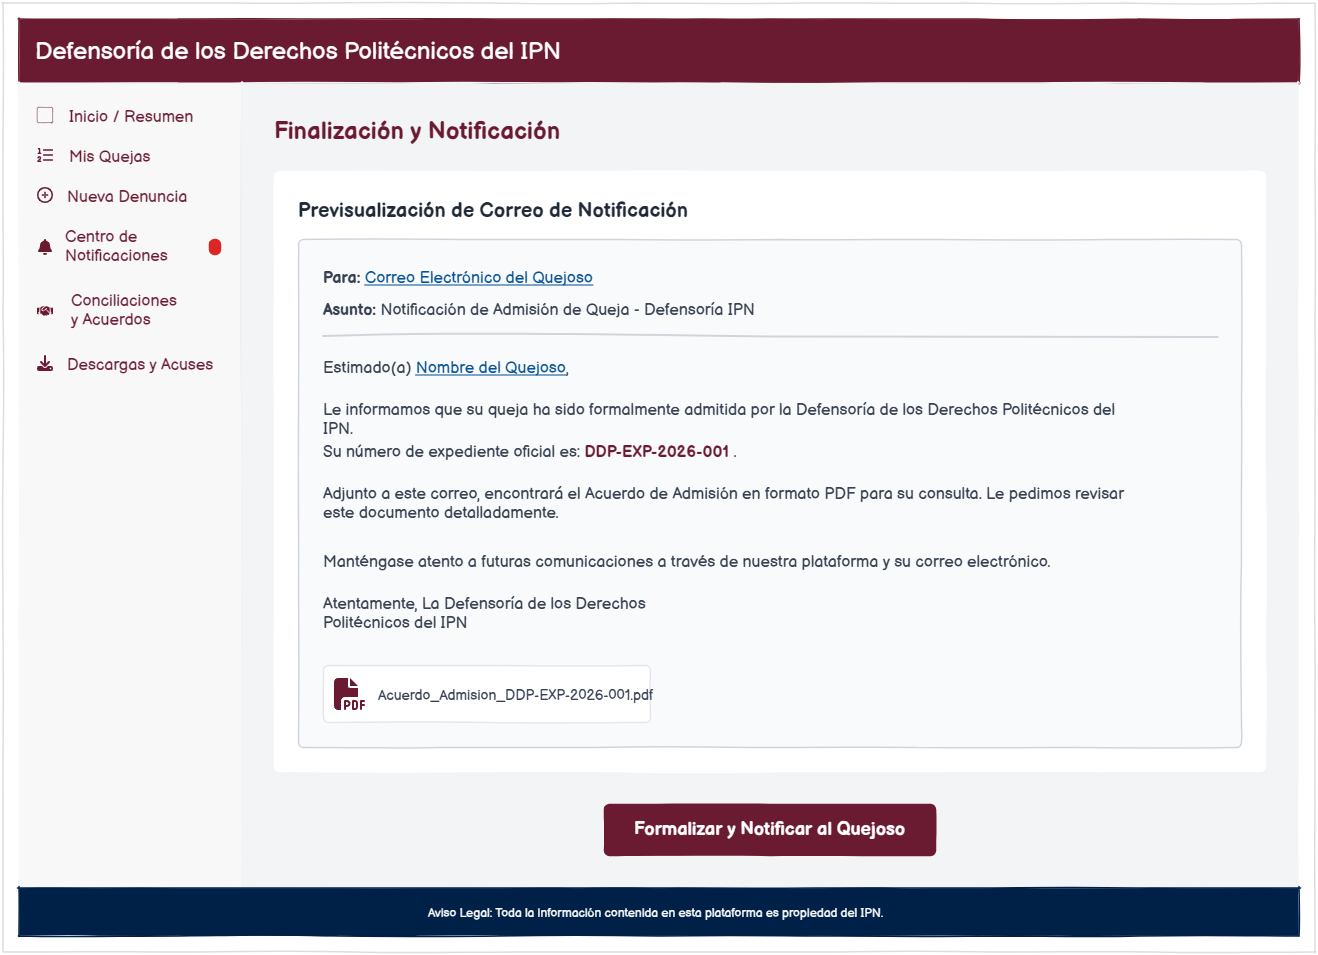
\includegraphics[width=0.65\textwidth]{imagenes/primercontacto/FormalizacionNotificacion.png}
\caption{MA-12: Interfaz de previsualización y notificación de admisión oficial.}
\label{fig:ma12_finalizacion_notificacion}
\end{figure}

\noindent \textbf{Descripción de la interfaz (MA-12):} \
Esta pantalla constituye el paso final del departamento de Primer Contacto antes de trasladar el expediente al área de instrucción en la Subdefensoría. Su propósito principal es garantizar la transparencia mediante una previsualización de la notificación oficial, permitiendo al analista verificar el cuerpo del correo electrónico y el número de expediente asignado. La interfaz muestra el archivo PDF del acuerdo de admisión vinculado y ofrece un botón de formalización que ejecuta simultáneamente el envío de la notificación y el cambio de estatus a "Admitida". De esta manera, se habilita el acceso al expediente para el siguiente departamento mientras el personal administrativo mantiene visibilidad sobre otras tareas pendientes en el entorno de gestión.

\clearpage

\end{appendices}